%%%%%%%%%%%%%%
%% Run LaTeX on this file several times to get Table of Contents,
%% cross-references, and citations.

%% If you have font problems, you may edit the w-bookps.sty file
%% to customize the font names to match those on your system.

%% w-bksamp.tex. Current Version: Feb 16, 2012
%%%%%%%%%%%%%%%%%%%%%%%%%%%%%%%%%%%%%%%%%%%%%%%%%%%%%%%%%%%%%%%%
%
%  Sample file for
%  Wiley Book Style, Design No.: SD 001B, 7x10
%  Wiley Book Style, Design No.: SD 004B, 6x9
%
%
%  Prepared by Amy Hendrickson, TeXnology Inc.
%  http://www.texnology.com
%%%%%%%%%%%%%%%%%%%%%%%%%%%%%%%%%%%%%%%%%%%%%%%%%%%%%%%%%%%%%%%%

%%%%%%%%%%%%%
% 7x10
%\documentclass{wileySev}

% 6x9
\documentclass{wileySix}

\usepackage{graphicx}
\usepackage{listings}
\usepackage{float}
\usepackage[urlcolor=blue, colorlinks=true]{hyperref}
\usepackage{textcomp}
\usepackage{gensymb}
\usepackage{color}
 
\definecolor{codegreen}{rgb}{0,0.6,0}
\definecolor{codegray}{rgb}{0.5,0.5,0.5}
\definecolor{codepurple}{rgb}{0.58,0,0.82}
\definecolor{backcolour}{rgb}{0.95,0.95,0.92}
 
\lstdefinestyle{mystyle}{
    backgroundcolor=\color{backcolour},   
    commentstyle=\color{codegreen},
    keywordstyle=\color{magenta},
    numberstyle=\tiny\color{codegray},
    stringstyle=\color{codepurple},
    basicstyle=\footnotesize,
    breakatwhitespace=false,         
    breaklines=true,                 
    captionpos=b,                    
    keepspaces=true,                 
    numbers=left,                    
    numbersep=5pt,                  
    showspaces=false,                
    showstringspaces=false,
    showtabs=false,                  
    tabsize=2,
    language=sh
}
 
\lstset{style=mystyle}

%%%%%%%
%% for times math: However, this package disables bold math (!)
%% \mathbf{x} will still work, but you will not have bold math
%% in section heads or chapter titles. If you don't use math
%% in those environments, mathptmx might be a good choice.

% \usepackage{mathptmx}

% For PostScript text
\usepackage{w-bookps}

%%%%%%%%%%%%%%%%%%%%%%%%%%%%%%%%%%%%%%%%%%%%%%%%%%%%%%%%%%%%%%%%
%% Other packages you might want to use:

% for chapter bibliography made with BibTeX
% \usepackage{chapterbib}

% for multiple indices
% \usepackage{multind}

% for answers to problems
% \usepackage{answers}

%%%%%%%%%%%%%%%%%%%%%%%%%%%%%%
%% Change options here if you want:
%%
%% How many levels of section head would you like numbered?
%% 0= no section numbers, 1= section, 2= subsection, 3= subsubsection
%%==>>
\setcounter{secnumdepth}{3}

%% How many levels of section head would you like to appear in the
%% Table of Contents?
%% 0= chapter titles, 1= section titles, 2= subsection titles, 
%% 3= subsubsection titles.
%%==>>
\setcounter{tocdepth}{2}

%% Cropmarks? good for final page makeup
%% \docropmarks

%%%%%%%%%%%%%%%%%%%%%%%%%%%%%%
%
% DRAFT
%
% Uncomment to get double spacing between lines, current date and time
% printed at bottom of page.
% \draft
% (If you want to keep tables from becoming double spaced also uncomment
% this):
% \renewcommand{\arraystretch}{0.6}
%%%%%%%%%%%%%%%%%%%%%%%%%%%%%%

%%%%%%% Demo of section head containing sample macro:
%% To get a macro to expand correctly in a section head, with upper and
%% lower case math, put the definition and set the box 
%% before \begin{document}, so that when it appears in the 
%% table of contents it will also work:

\newcommand{\VT}[1]{\ensuremath{{V_{T#1}}}}

%% use a box to expand the macro before we put it into the section head:

\newbox\sectsavebox
\setbox\sectsavebox=\hbox{\boldmath\VT{xyz}}

%%%%%%%%%%%%%%%%% End Demo


\begin{document}


\booktitle{Cerdas Menguasai Git}
\subtitle{Dalam 24 Jam}

\authors{Rolly M. Awangga\\
\affil{Informatics Research Center}
%Floyd J. Fowler, Jr.\\
%\affil{University of New Mexico}
}

\offprintinfo{Cerdas Menguasai Git, First Edition}{Rolly M. Awangga}

%% Can use \\ if title, and edition are too wide, ie,
%% \offprintinfo{Survey Methodology,\\ Second Edition}{Robert M. Groves}

%%%%%%%%%%%%%%%%%%%%%%%%%%%%%%
%% 
\halftitlepage

\titlepage


\begin{copyrightpage}{2019}
%Survey Methodology / Robert M. Groves . . . [et al.].
%\       p. cm.---(Wiley series in survey methodology)
%\    ``Wiley-Interscience."
%\    Includes bibliographical references and index.
%\    ISBN 0-471-48348-6 (pbk.)
%\    1. Surveys---Methodology.  2. Social 
%\  sciences---Research---Statistical methods.  I. Groves, Robert M.  II. %
%Series.\\
%
%HA31.2.S873 2007
%001.4'33---dc22                                             2004044064
\end{copyrightpage}

\dedication{`Jika Kamu tidak dapat menahan lelahnya belajar, 
Maka kamu harus sanggup menahan perihnya Kebodohan.'
~Imam Syafi'i~}

\begin{contributors}
\name{Rolly Maulana Awangga,} Informatics Research Center., Politeknik Pos Indonesia, Bandung,
Indonesia



\end{contributors}

\contentsinbrief
\tableofcontents
%\listoffigures
%\listoftables
%\lstlistoflistings


\begin{foreword}
Sepatah kata dari Kaprodi, Kabag Kemahasiswaan dan Mahasiswa
\end{foreword}

\begin{preface}
Buku ini diciptakan bagi yang awam dengan git sekalipun.

\prefaceauthor{R. M. Awangga}
\where{Bandung, Jawa Barat\\
Februari, 2019}
\end{preface}


\begin{acknowledgments}
Terima kasih atas semua masukan dari para mahasiswa agar bisa membuat buku ini 
lebih baik dan lebih mudah dimengerti.

Terima kasih ini juga ditujukan khusus untuk team IRC yang 
telah fokus untuk belajar dan memahami bagaimana buku ini mendampingi proses 
Intership.
\authorinitials{R. M. A.}
\end{acknowledgments}

\begin{acronyms}
\acro{ACGIH}{American Conference of Governmental Industrial Hygienists}
\acro{AEC}{Atomic Energy Commission}
\acro{OSHA}{Occupational Health and Safety Commission}
\acro{SAMA}{Scientific Apparatus Makers Association}
\end{acronyms}

\begin{glossary}
\term{git}Merupakan manajemen sumber kode yang dibuat oleh linus torvald.

\term{bash}Merupakan bahasa sistem operasi berbasiskan *NIX.

\term{linux}Sistem operasi berbasis sumber kode terbuka yang dibuat oleh Linus Torvald
\end{glossary}

\begin{symbols}
\term{A}Amplitude

\term{\hbox{\&}}Propositional logic symbol 

\term{a}Filter Coefficient

\bigskip

\term{\mathcal{B}}Number of Beats
\end{symbols}


%%%%%%%%%%%%%%%%%%Isi Buku_

\chapter{Chapter 1}
%\section{Dinda Anik Masruro - 1184003}
\subsection{Teori}
\begin{enumerate}

	\item Definisi Kecerdasan Buatan
	\hfill\break
	Kecerdasan Buatan atau biasa disebut dengan istilah AI (Artificial Intelligence). Kecerdasan Buatan adalah salah satu bidang studi yang berhubungan dengan pemanfaatan mesin untuk memecahkan persoalan yang rumit dengan cara lebih manusiawi dan lebih bisa di pahami oleh manusia. Kecerdasan buatan makin canggih dengan kemampuan komputer dalam memperbarui pengetahuannya dengan banyaknya testing dan perkembangan target analisa. Untuk kecerdasan buatan ada banyak contoh dan jenisnya. Salah satu contoh yang paling terkenal dari Artificial Intelligence ialah Google Assistant. Google Assistant digunakan untuk kemudahan user dalam menemukan berbagai hal maupun penyetingan langsung terhadap smartphone yang digunakan dan masih banyak lagi.

	\item Sejarah dan Perkembangan
	\hfill\break
    Pada tahun 1943, pekerjaan pertama yang dikenal sebagai AI atau \textit{Artificial Intellegent} telah dikemukakan oleh Warren McCulloch dan juga Walter Pits yang dinamakan sebagai artificial neurons. Kemudian pada tahun 1955, Allen Newell dan Herbert A. Simon membuat program kecerdasan buatan pertama yang dinamakan Logic Theorist. Lalu pada tahun 1972, robot pertama dibuat di jepang dengan nama Wabot-1 dengan kecerdasan buatan. Pada tahun 1980, muncul bidang baru dari kecerdasan buatan yaitu Expert System yang membantu dalam pemberian keputusan. Kemudian pada tahun 1997, IBM deep blue mengalahkan juara catur dunia Gary Kasparov dan menjadi komputer pertama yang mengalahkannya. Tahub 2006, perusahaaan sudah mulai menerapkan kecerdasan buatan pada produknya seperti Netflix dan Twitter. Tahun 2018, Project Debater dari IBM melakuakn debat tentang topik yang kompleks dan berakhir dengan hasil memuaskan.
	
	\item Kecerdasan buatan terbagi atas beberapa metode yaitu:
	\hfill\break
	Supervised learning,  Klasifikasi, Regresi,Unsupervised Learning, Dataset, Trainingset dan juga Testingset.
	\begin{itemize}
		\item Supervised Learning
		\hfill\break
	Supervised Learning adalah sebuah tipe learning yang mempunyai variable input dan variable output, tipe ini juga menggunakan satu algoritma atau lebih dari satu algoritma yang digunakan untuk mempelajari fungsi  pemetaan dari input ke output.
		\item Klasifikasi
		\hfill\break
		Klasifikasi merupakan suatu kegiatan dari penggolongan atau pengelompokkan. Tetapi secara umum klasifikasi merupakan suatu kegiatan yang dapat mengelompokkan benda-benda yang memiliki beberapa ciri-ciri yang sama dan memisahkan benda yang tidak sama. 
		\item Regresi
		\hfill\break
        Regresi adalah metode analisis statistik yang digunakan untuk dapat melihat efek antara dua atau lebih variabel. Hubungan variabel dalam pertanyaan adalah fungsional yang diwujudkan dalam bentuk model matematika. Dalam analisis regresi, variabel dibagi menjadi dua jenis, yaitu variabel respons atau yang biasa disebut variabel dependen dan variabel independen atau dikenal sebagai variabel independen. Ada beberapa jenis analisis regresi, yaitu regresi sederhana yang mencakup linear sederhana dan regresi non-linear sederhana dan regresi berganda yang mencakup banyak linier atau non-linear berganda. Analisis regresi digunakan dalam pembelajaran mesin pembelajaran dengan metode pembelajaran terawasi.
		\item Unsupervised Learning 
		\hfill\break
        Unsupervised Learning merupakan pelatihan algoritma kecerdasan buatan (AI) menggunakan informasi yang tidak diklasifikasikan atau diberi label dan memungkinkan algoritma untuk bertindak atas informasi tersebut tanpa bimbingan. Dalam Unsupervised Learning, sistem AI dapat mengelompokkan informasi yang tidak disortir berdasarkan persamaan dan perbedaan meskipun tidak ada kategori yang disediakan.
		\item Data set
		\hfill\break
        Data set adalah objek yang merepresentasikan data dan relasinya di memory. Strukturnya mirip dengan data di database. Dataset berisi koleksi dari datatable dan datarelation.
		\item Training Set
		\hfill\break
    	Training set merupakan bagian dari data set yang di latih untuk membuat prediksi atau menjalankan fungsi dari algoritma ML lain sesuai dengan masing-masing. Memberikan instruksi melalui algoritma sehingga mesin yang di praktikkan dapat menemukan korelasinya sendiri.	
		\item Testing Set
		\hfill\break
        Testing set adalah bagian dari data set yang di uji untuk melihat akurasinya, atau dengan kata lain untuk melihat kinerjanya.
	\end{itemize}
\end{enumerate}
\subsection{Praktek}
\begin{enumerate}
	\item Instalasi Library scikit dari Anaconda, mencoba kompilasi dan uji coba ambil contoh kode dan lihat variabel explorer
	\hfill\break
	\begin{figure}[h]
		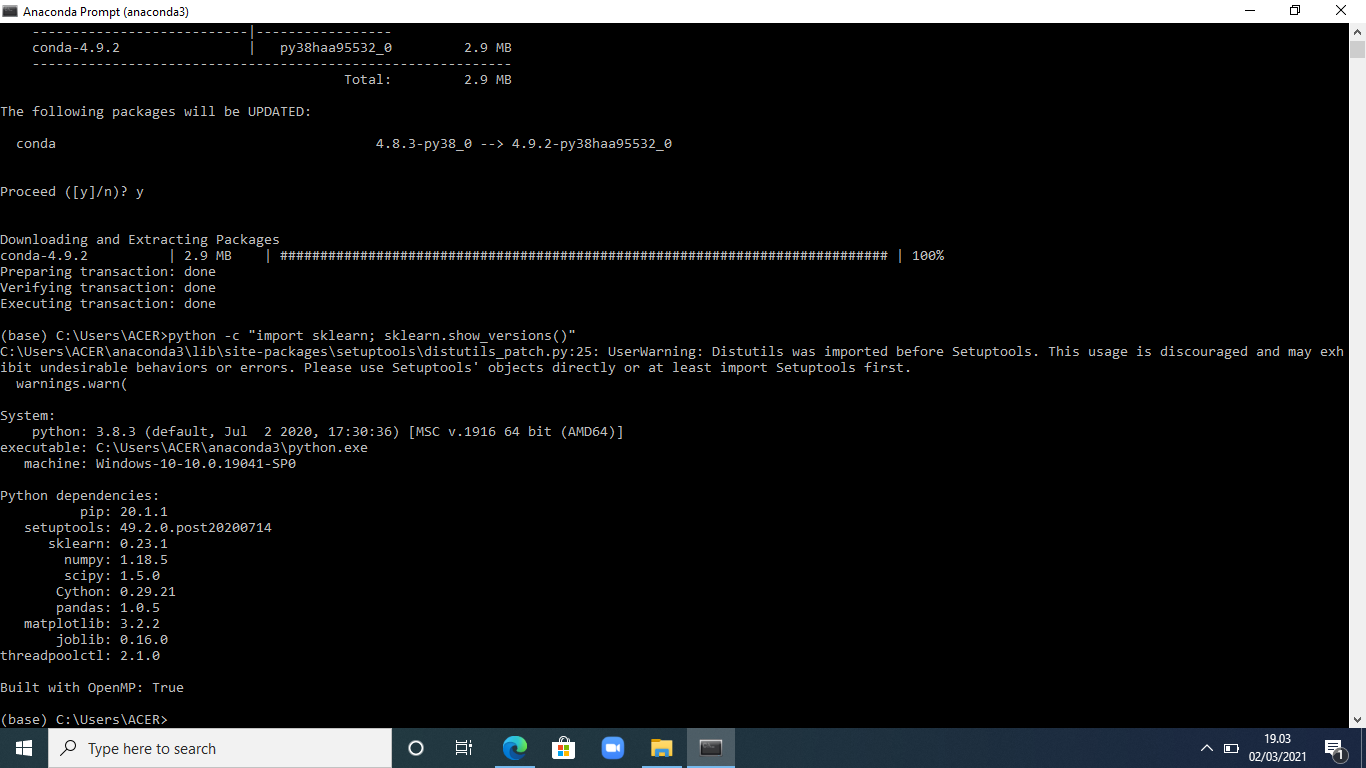
\includegraphics[width=10cm]{figures/1184003/chapter1/1.png}
		\centering
		\caption{Instalasi Library Scikit Learn}
	\end{figure}
	\begin{figure}[h]
		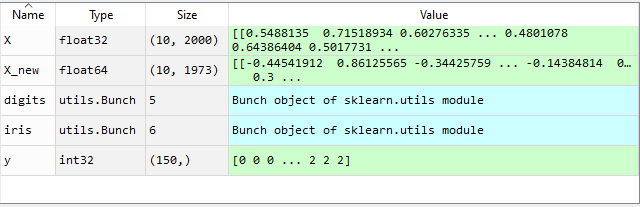
\includegraphics[width=10cm]{figures/1184003/chapter1/2.PNG}
		\centering
		\caption{Isi Variabel Explorer}
	\end{figure}
	\newpage\item Uji coba loading an example dataset
	\hfill\break
\lstinputlisting[firstline=7, lastline=16]{src/tugas1.py}
\item Uji coba Learning dan predicting
	\hfill\break
	\lstinputlisting[firstline=17, lastline=32]{src/tugas1.py}
\item Uji coba Model Persistence
	\hfill\break
	\lstinputlisting[firstline=35, lastline=63]{src/tugas1.py}	
	\item Uji coba Conventions
	\hfill\break
	\lstinputlisting[firstline=64, lastline=82]{src/tugas1.py}
	\end{enumerate}
	\subsection{Penanganan Error}
\begin{enumerate}
	\item ScreenShoot Error
	\begin{figure}[h]
		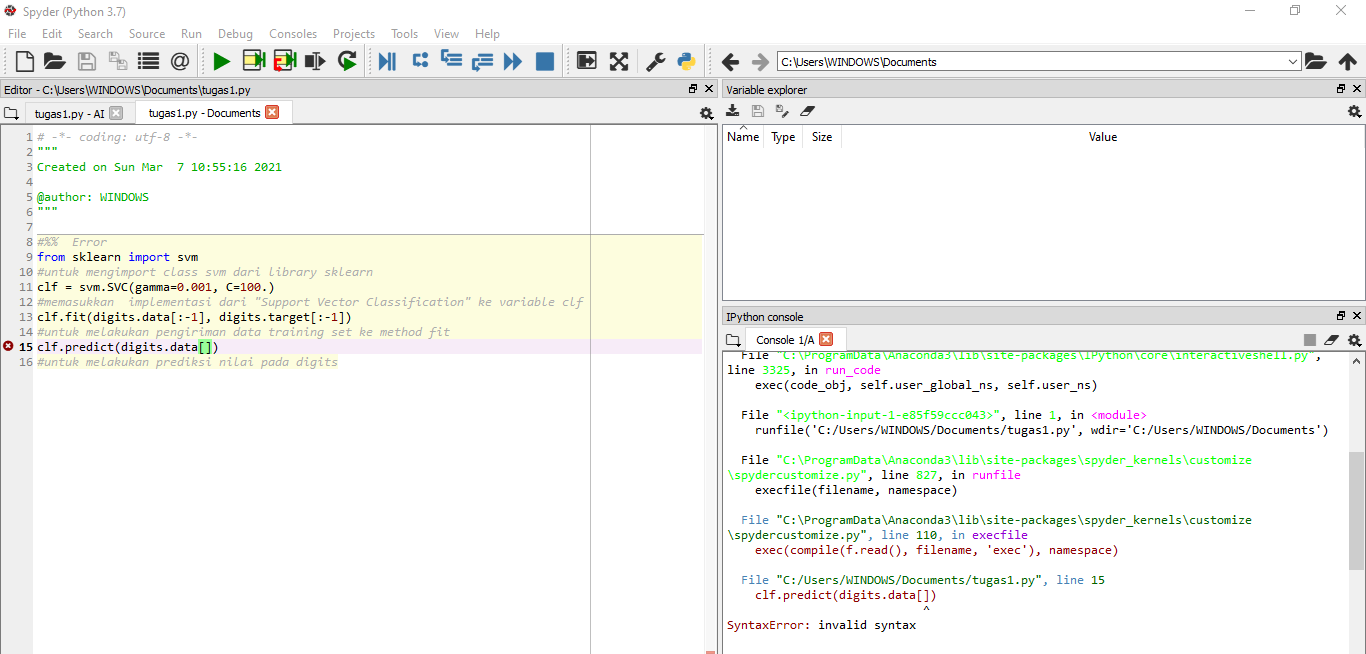
\includegraphics[width=10cm]{figures/1184003/chapter1/3.PNG}
		\centering
		\caption{Name Error}
	\end{figure}
	\newpage\item Tuliskan Kode Error dan Jenis Error
	\hfill\break
	\lstinputlisting[firstline=83, lastline=91]{src/tugas1.py}
\hfill\break
	\item Cara Penangan Error
\hfill\break Tambahkan prediksi nilainya agar kode program dapat terbaca
	\end{enumerate}
	\subsection{Bukti Tidak Plagiat}
\begin{figure}[h]
	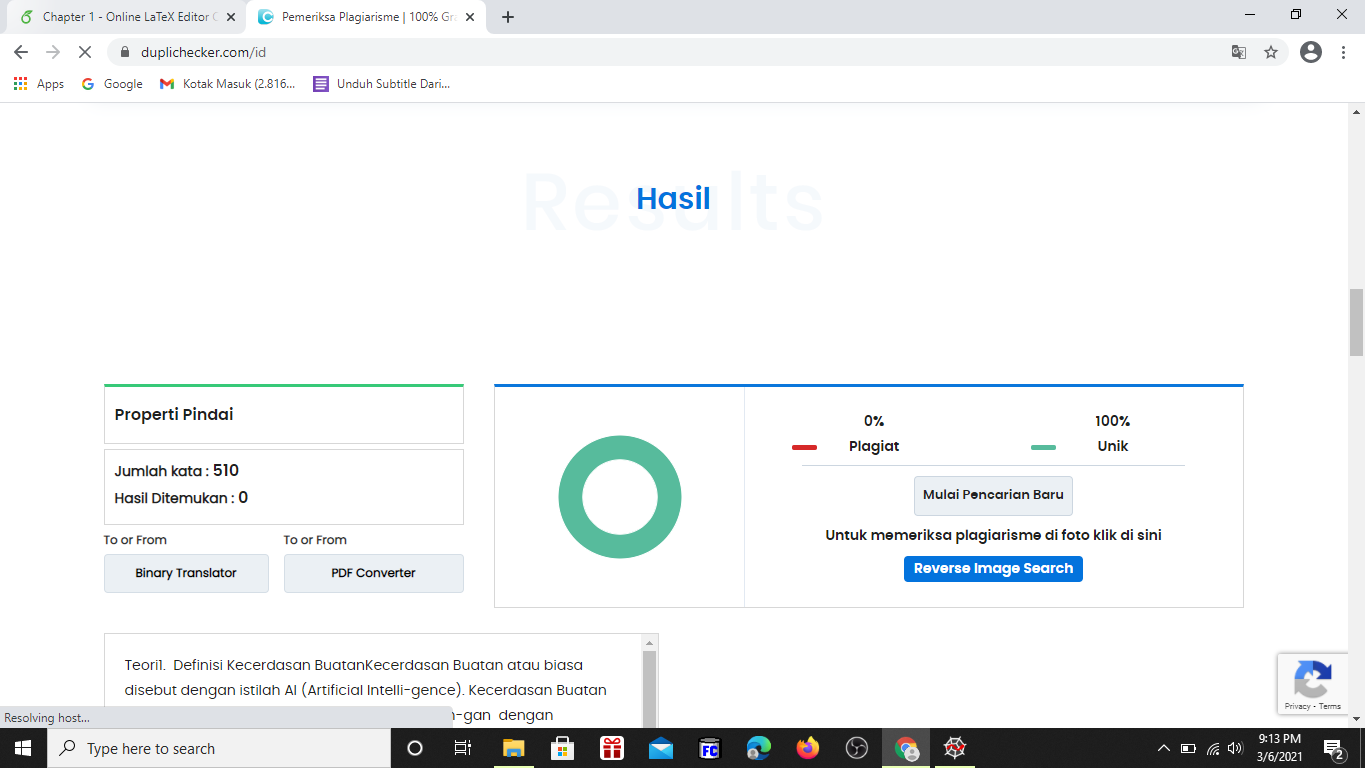
\includegraphics[width=10cm]{figures/1184003/chapter1/4.png}
	\centering
	\caption{Bukti Tidak Melakukan Plagiat Chapter 1}
\end{figure}
%\section{1184006 - Murnia Lestari}
\subsection{Teori}
\begin{enumerate}

	\item Definisi Kecerdasan Buatan
	\hfill\break
	Kecerdasan Buatan atau Artifical Inteligence yang terdiri dari kata cerdas dan buatan. Cerdas artiya cepat dan tepat.  Sedangkan buatan artinya sesuatu yang sengaja dibuat dengan tujuan tertentu. Jadi kecerdasan buatan merupakan sebuah sistem yang disimulasikan dari kecerdasan yang dipunyai oleh manusia. Sehingga sistem ini akan melakukan pelkerjaan-pekerjaan yang umumnya dikerjakan oleh manusia secara cepat dan tepat seperti yang dilakukan oleh manusia. Point-point penting yang terdapat  dalam proses kecerdasan buatan adalah learning,reasoning dan self correction.

	\item Sejarah dan Perkembangan
	\hfill\break
Kecerdasan buatan bermula pada tahun 1940-an yang bermula dari kemunculan komputer. Kemudia pada tahun 1943 McMulloh dan Pitts pada tahun 1943 mempunyai usul untuk membuat model matematis yang bernama percepton dari neurin yang ada didalam otak. Pada tahun 1950 terbuatlah mesin turing yang mencoba menjawab “dapatkah computer berpikir” yang terdapat pada paper Alan Turing. Pada tahun 1955 akhir,Newell dan simon mengembangkan The Logic Theorist yaitu program kecerdasan buatan yang pertama. Pada tahun 1956 dari Massacuhetts Institute of Technology yaitu John McCharty yang dianggap sebagai bapak dari kecerdasan buatan atau AI menyelenggarakan konferensi untuk para ahli komputer dengan nama “ The Dartmouth summer research project on artifical intelligence. Pada tahun 1960-1970 muncullah “classical AI” yang merupakan diskusi mengenai bagaimana komputer dapat meniru dengan detail kemmapuan otak manusia. Dan pada tahun 1980 merupakan titik dimna kecerdasan buatan berkembang karena komputer dapat diperoleh dengan harga yag lebih murah.
	

	\item Kecerdasan buatan terbagi atas beberapa metode yaitu:
	\hfill\break
	Supervised learning,  Klasifikasi, Regresi,Unsupervised Learning, Dataset, Trainingset dan juga Testingset.
	\begin{itemize}
		\item Supervised Learning
		\hfill\break
	Supervised Learning	merupakan algoritma yang memiliki attribut tambahan seperti x dan y yang ingin diprediksi.
		\item Klasifikasi
		\hfill\break
		Klasifikasi merupakan sampel yang dimiliki oleh dua atau lebih kelas yang dikelompokkan yang disesuaikan berdasarkan ukuran kemiripan atau jarak yang melekat. 
		\item Regresi
		\hfill\break
Regresi	merupakan sebuah prediksi apabila hasil atau output yang diinginkan terdiri dari satu atau lebih variable contionous.
		\item Unsupervised Learning 
		\hfill\break
Unsupervised Learning  merupakan	algoritma yang tidak memiliki attribut tambahan yang akan diprediksi
		\item Data set
		\hfill\break
Data set	merupakan kondisi dimana hanya terdapat inputan data tanpa memiliki viariasi output yang sesuai
		\item Training Set
		\hfill\break
	Training Set	merupakan bagian dari data set yang digunakan untuk mempelajari beberapa properti		
		\item Testing Set
		\hfill\break
Testing Set	merupakan bagian data set yang digunakan untuk pengujian dari properti yang dipelajari
	\end{itemize}
\end{enumerate}
\subsection{Praktek}
\begin{enumerate}
	\item Instalasi Library scikit dari Anaconda, mencoba kompilasi dan uji coba ambil contoh kode dan lihat variabel explorer
	\hfill\break
	\begin{figure}[h]
		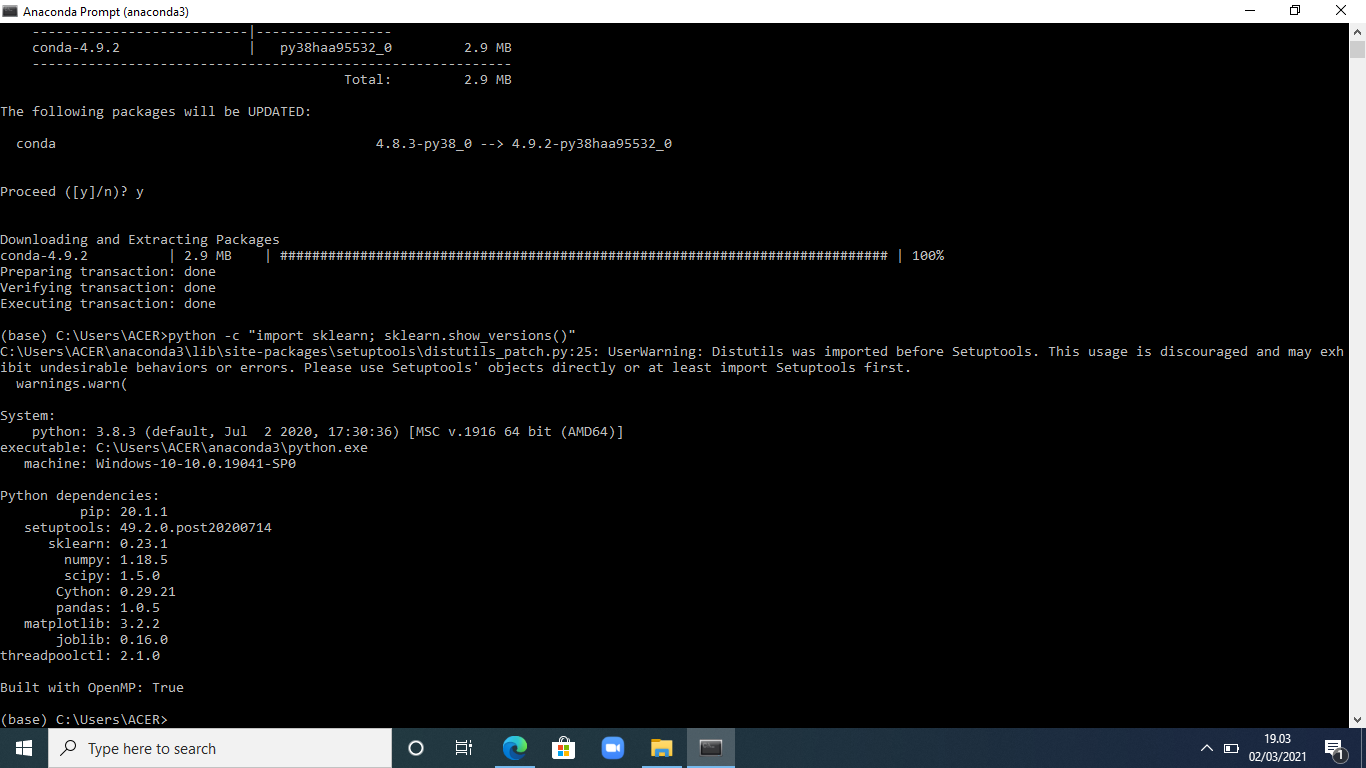
\includegraphics[width=10cm]{figures/1184006/chapter1/01.png}
		\centering
		\caption{Instalasi Library Scikit Learn}
	\end{figure}
	\begin{figure}[h]
		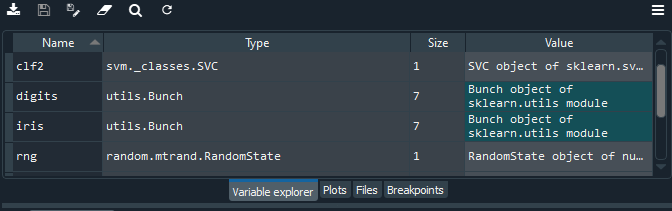
\includegraphics[width=10cm]{figures/1184006/chapter1/02.PNG}
		\centering
		\caption{Isi Variabel Explorer}
	\end{figure}
	\newpage\item Uji coba loading an example dataset
	\hfill\break
\lstinputlisting[firstline=7, lastline=16]{src/1184006/chapter1/tugas1.py}
\item Uji coba Learning dan predicting
	\hfill\break
	\lstinputlisting[firstline=17, lastline=32]{src/1184006/chapter1/tugas1.py}
\item Uji coba Model Persistence
	\hfill\break
	\lstinputlisting[firstline=35, lastline=63]{src/1184006/chapter1/tugas1.py}
	\item Uji coba Conventions
	\hfill\break
	\lstinputlisting[firstline=64, lastline=82]{src/1184006/chapter1/tugas1.py}
	\end{enumerate}
	\subsection{Penanganan Error}
\begin{enumerate}
	\item ScreenShoot Error
	\begin{figure}[h]
		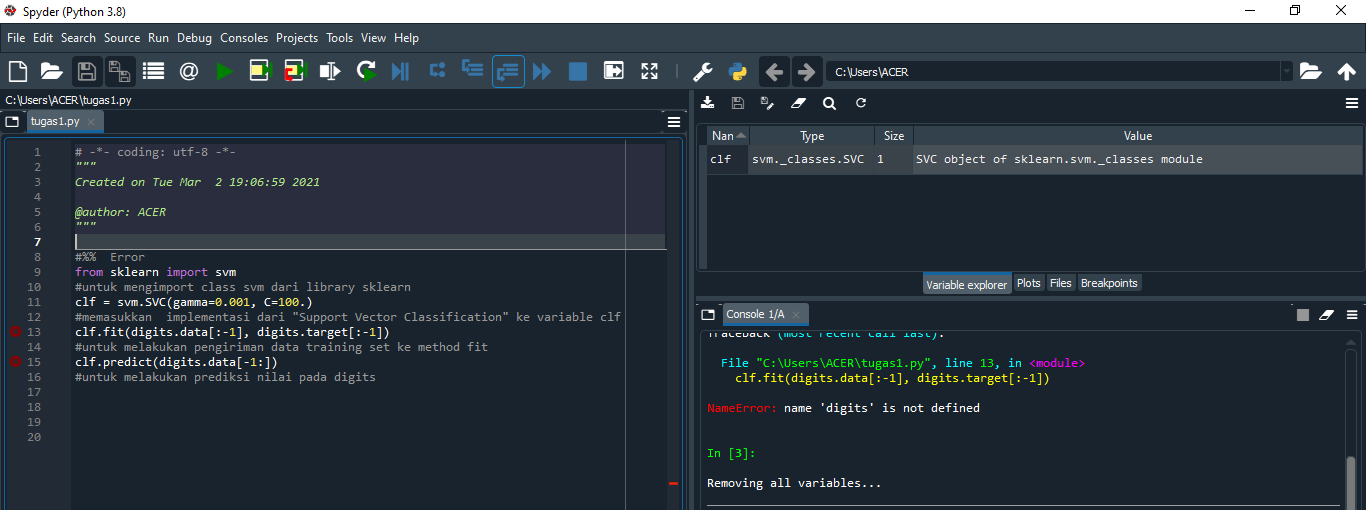
\includegraphics[width=10cm]{figures/1184006/chapter1/03.PNG}
		\centering
		\caption{Name Error}
	\end{figure}
	\newpage\item Tuliskan Kode Error dan Jenis Error
	\hfill\break
	\lstinputlisting[firstline=83, lastline=91]{src/1184006/chapter1/tugas1.py}
\hfill\break
	\item Cara Penangan Error
\hfill\break Tambahkan variabel digits agar kode program dapat terbaca
	\end{enumerate}
	\subsection{Bukti Tidak Plagiat}
\begin{figure}[h]
	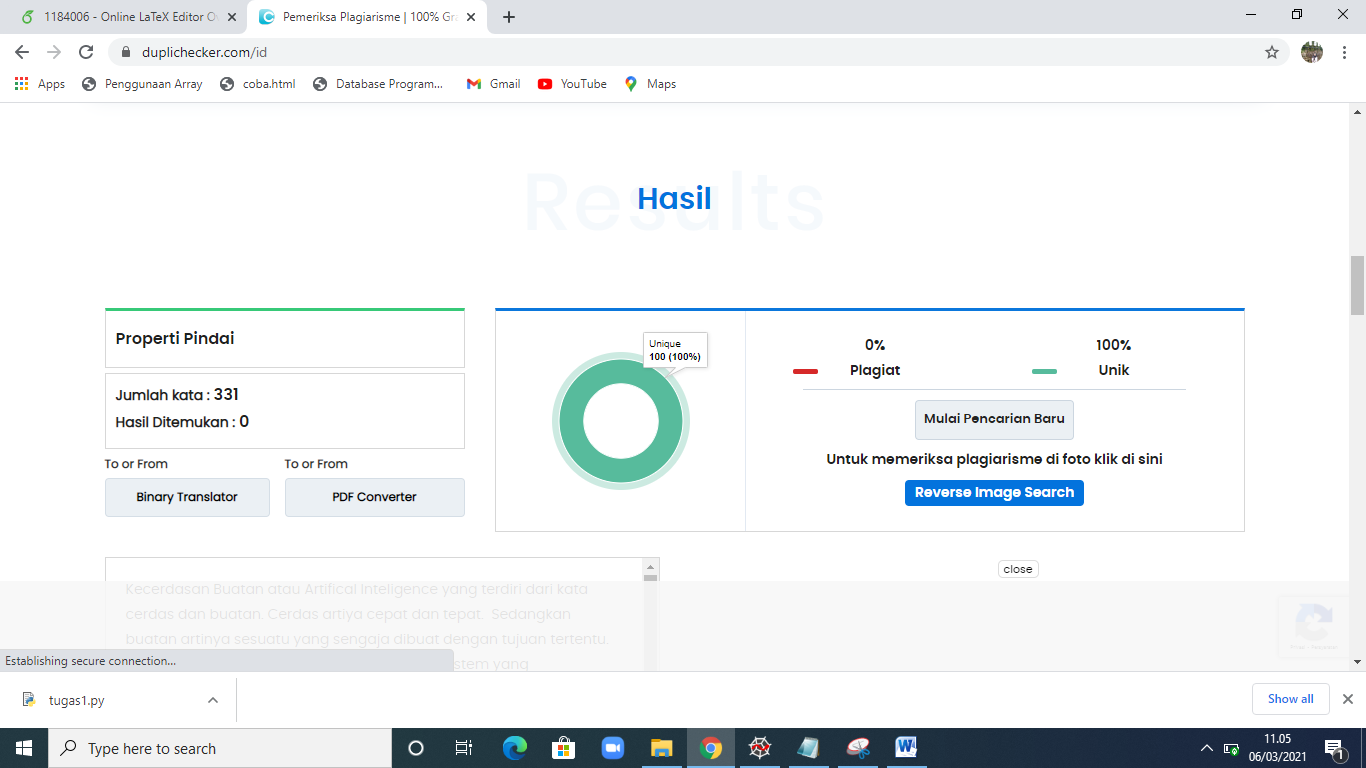
\includegraphics[width=10cm]{figures/1184006/chapter1/04.png}
	\centering
	\caption{Bukti Tidak Melakukan Plagiat Chapter 1}
\end{figure}
%\section{1184071 - Annisa Khairani Febrianti}
\subsection{Teori}
\begin{enumerate}
	\item Definisi Kecerdasan Buatan (AI)
	\hfill\break
	Kecerdasan Buatan atau \textit{Artificial Intelligence} (AI) merupakan teknik meniru kecerdasan yang dimiliki oleh makhluk hidup maupun benda mati untuk menyelesaikan suatu masalah. Atau dapat di definisikan sebagai salah satu cabang Ilmu pengetahuan yang berkaitan dengan pemanfaatan mesin untuk menyelesaikan persoalan rumit dengan menggunakan cara yang lebih manusiawi. Adapun contoh sederhana penerapan kecerdasan buatan adalah SIRI, bagi pengguna iphone atau \textit{IOS} pasti sudah tidak asing dengan SIRI yang
    seringkali diartikan sebagai asisten pribadi pengguna IOS dalam melakukan hal-hal tertentu untuk penggunanya.

	\item Perkembangan dan Sejarah AI
	\hfill\break
	Pada tahun 1956 merupakan tahun pertama kali muncul istilah AI atau \textit{Artificial Intellegent} yang dikemukakan oleh \textbf{John McCarthy} di Konferensi Darthmouth.Penggunaan AI begitu popular dari tahun ke tahun. Pada tahun 1950-an merupakan tahap dimana riset awal proyek AI yang tujuan untuk eksplorasi topik penyelesaian persoalan dan metode simbolik.Selanjutnya Pada tahun 1959, Dari IBM yang bernama \textbf{Nathaniel Rochester} bersama beberapa mahasiswa lainnya mengeluarkan program kecerdasan buatan yaitu \textit{Geometry Theorm Prover}. Lalu pada tahun 1960-an Departemen Pertahanan yang berasal dari Amerika Serikat memiliki keinginan dalam melatih dan mengembangkan komputer supaya memiliki nalar yang menyerupai manusia secara dasar. Kemudian Pada tahun 1963, program yang mampu menyelesaikan masalah integral tertutup untuk mata kuliah Kalkulus dibuat dengan \textbf{James Slagle}. Pada tahun 1970-an, adanya suatu keberhasilan proyek DARPA \textit{(Defence Advanced Research Project Agency)} dengan mampu menyelesaikan studi kasus tentang pemetaan jalan. Selanjutnya Pada tahun 1986, program analogi yang digunakan dalam pemecahan masalah analogi geometris yang ada pada tes IQ dibuatan oleh \textbf{Tom Evan}. Dari tahun 1980an AI kemudian mulai berkembang dibidang idustri dan mulai berkiprah hingga saat ini dimana para ilmuan berlomba-lomba untuk menciptakan AI yang bermanfaat pada kehidupan sekarang atau dimasa depan nanti. Setelah itu pada awal abad ke 21 atau lebih tepatnya pada tahun 2003, DARPA berhasil untuk menciptakan asisten pribadi yang cerdas. Sejak saat itu lah teknologi AI terus berkembang sangat bagus dan sampai saat ini AI tersebutlebih menjurus pada program yang lebih detail dan kompleks dengan penerapan struktur algoritma dari pembelajaran secara mendalam atau \textit{deep learning} yaitu AI yang dikembangkan bisa mengerjakan persoalan dan memberi solusi yang lebih kompleks dengan kondisi yang lebih beragam.

	\item Kecerdasan buatan (AI) terbagi menjadi beberapa metode yaitu:
	\hfill\break
	Supervised learning,  Klasifikasi, Regresi,Unsupervised Learning, Dataset, Trainingset dan juga Testingset.
	\begin{itemize}
		\item Supervised Learning
		\hfill\break
	Supervised learning merupakan suatu pembelajaran dengan adanya pengawas atau bisa disebut dengan supervisor. Supervisor merupakan suatu label yang ada di setiap data nya. Kemudian label tersebut berisi tag dari data yang ditambah ke dalam model pembelajaran mesin atau lebih trend disebut dengan \textbf{machine learning model}. Bisa diilustrasikan seperti gambar apel di tag “apel” dari masing-masing gambar tersebut apel dan gambar pir di tag “pir”dari masing-masing gambar pir. Lalu Machine learning memiliki berapa kategori berupa clasification (“apel”, “pir”, dsb) dan regression ( tinggi badan, berat badan, dsb).
		\item Klasifikasi
		\hfill\break
		Klasifikasi merupakan sampel yang dimiliki oleh dua atau lebih kelas yang dikelompokkan yang disesuaikan berdasarkan ukuran kemiripan atau jarak yang melekat. 
		\item Regresi
		\hfill\break
    Regresi	merupakan sebuah prediksi apabila hasil atau output yang diinginkan terdiri dari satu atau lebih variable contionous.
		\item Unsupervised Learning 
		\hfill\break
Unsupervised learning merupakan suatu pembelajaran tanpa adanya sebuah pengawasan dan tidak menggunakan label untuk bisa memprediksi target variable. Unsupervised learning lebih mengelompokan tentang kesamaan ataupun kemiripan dari attribut yang sudah diinputkan. Apabila attribut dan sifat dari data variable yang diproses ternyata memiliki kemiripan, maka akan dijadikan
satu kelompok (clustering). Dan akan menimbulkan beberapa bagian kelompok (cluster). Jumlah cluster bisa tidak terbatas. Dari kelompok tersebut model melabelkan, dan jika data baru akan di prediksi, itu akan diproses untuk mencocokan kelompok yang memiliki kemiripan feature. unsupervised learning tidak punya outcome spesifik seperti supervise learning karena tidak adanya sebuah label dasar.
\hfill\break
\textbf{Dapat disimpulkan Jika Supervised learning tentang atribut atau label yang sudah ada dari kategori yang diinginkan berbeda dengan unservised learning dimana unsupervised menggunakan kesamaan dari attribut yang dimiliki. Jika attribut dan sifat dari data feature yang diekstrak memiliki
kemiripan, maka akan dikelompokan kedalam \textit{(clustering)}. Sehingga hal ini
akan menimbulkan kelompok \textit{(cluster)}. Jumlah cluster bisa unlimited atau tidak terbatas}.
		\item Data Set
		\hfill\break
Data Set merupakan kumpulan sampel yang sudah dikumpulkan dan bersifat
homogen. Salah satu contohnya yaitu Seorang anak ingin bermain Voli, tetapi keputusannya untuk bermain voli tersebut tergantung pada variable yang ditentukan contohnya jarak kaki dari garis, atau tinggi net sehingga variable ini disebut dengan fitur dalam sebuah permainan.
		\item Training Set
		\hfill\break
Data yang digunakan untuk bisa melakukan klasifikasi ataupun prediksi,Dengan adanya data training maka akan didapatkan sebuah model regresi.		
		\item Testing Set
		\hfill\break
Testing Set digunakan untuk menguji kebenaran dari sebuah model data.Adapun Testing data berisi \textit{unseen example} merupakan contoh yang tidak ada didalam training set.
	\end{itemize}
\end{enumerate}
\subsection{Praktek}
\begin{enumerate}
	\item Instalasi Library scikit dari Anaconda, mencoba kompilasi dan uji coba ambil contoh kode dan lihat variabel explorer
	\hfill\break
	\begin{figure}[h]
		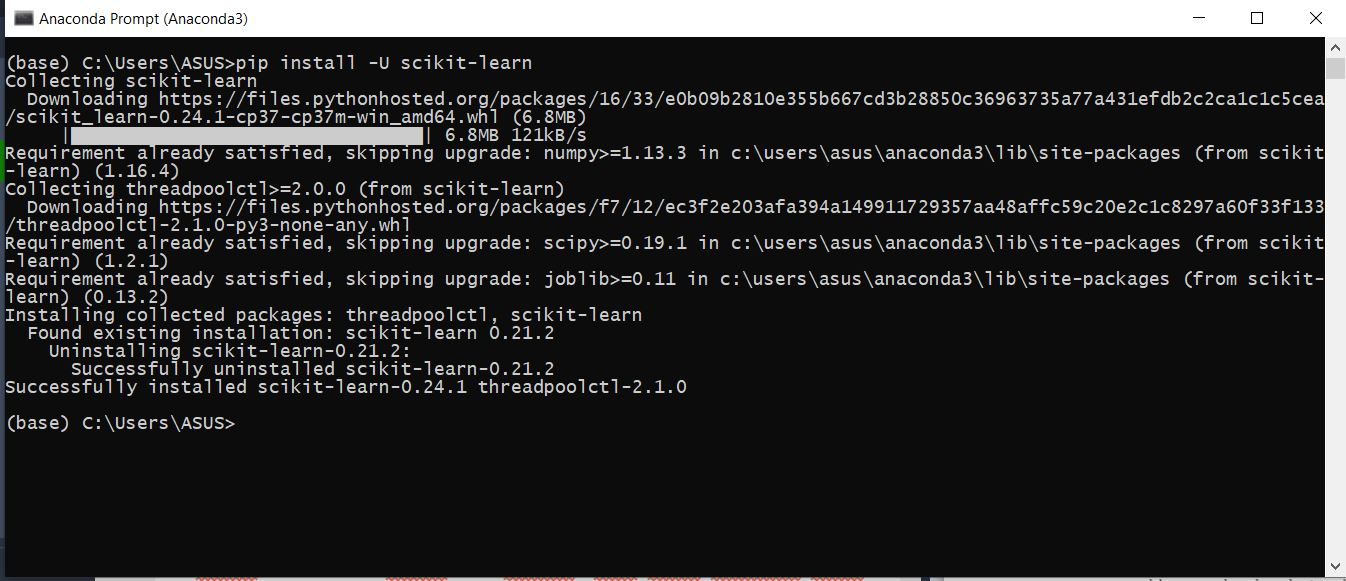
\includegraphics[width=12cm]{figures/1184071/chapter1/1.JPG}
		\centering
		\caption{Instalasi Library Scikit Learn}
	\end{figure}
	\begin{figure}[h]
		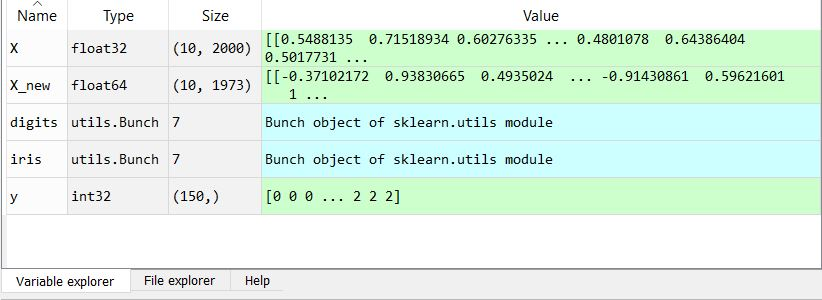
\includegraphics[width=15cm]{figures/1184071/chapter1/2.JPG}
		\centering
		\caption{Isi Variabel Explorer}
	\end{figure}
	\newpage\item Uji coba loading an example dataset
	\hfill\break
\lstinputlisting[firstline=7, lastline=16]{src/tugas1.py}
\item Uji coba Learning dan predicting
	\hfill\break
	\lstinputlisting[firstline=17, lastline=32]{src/tugas1.py}
\item Uji coba Model Persistence
	\hfill\break
	\lstinputlisting[firstline=35, lastline=63]{src/tugas1.py}	
	\item Uji coba Conventions
	\hfill\break
	\lstinputlisting[firstline=64, lastline=82]{src/tugas1.py}
	\end{enumerate}
	\subsection{Penanganan Error}
\begin{enumerate}
	\item ScreenShoot Error
	\begin{figure}[h]
		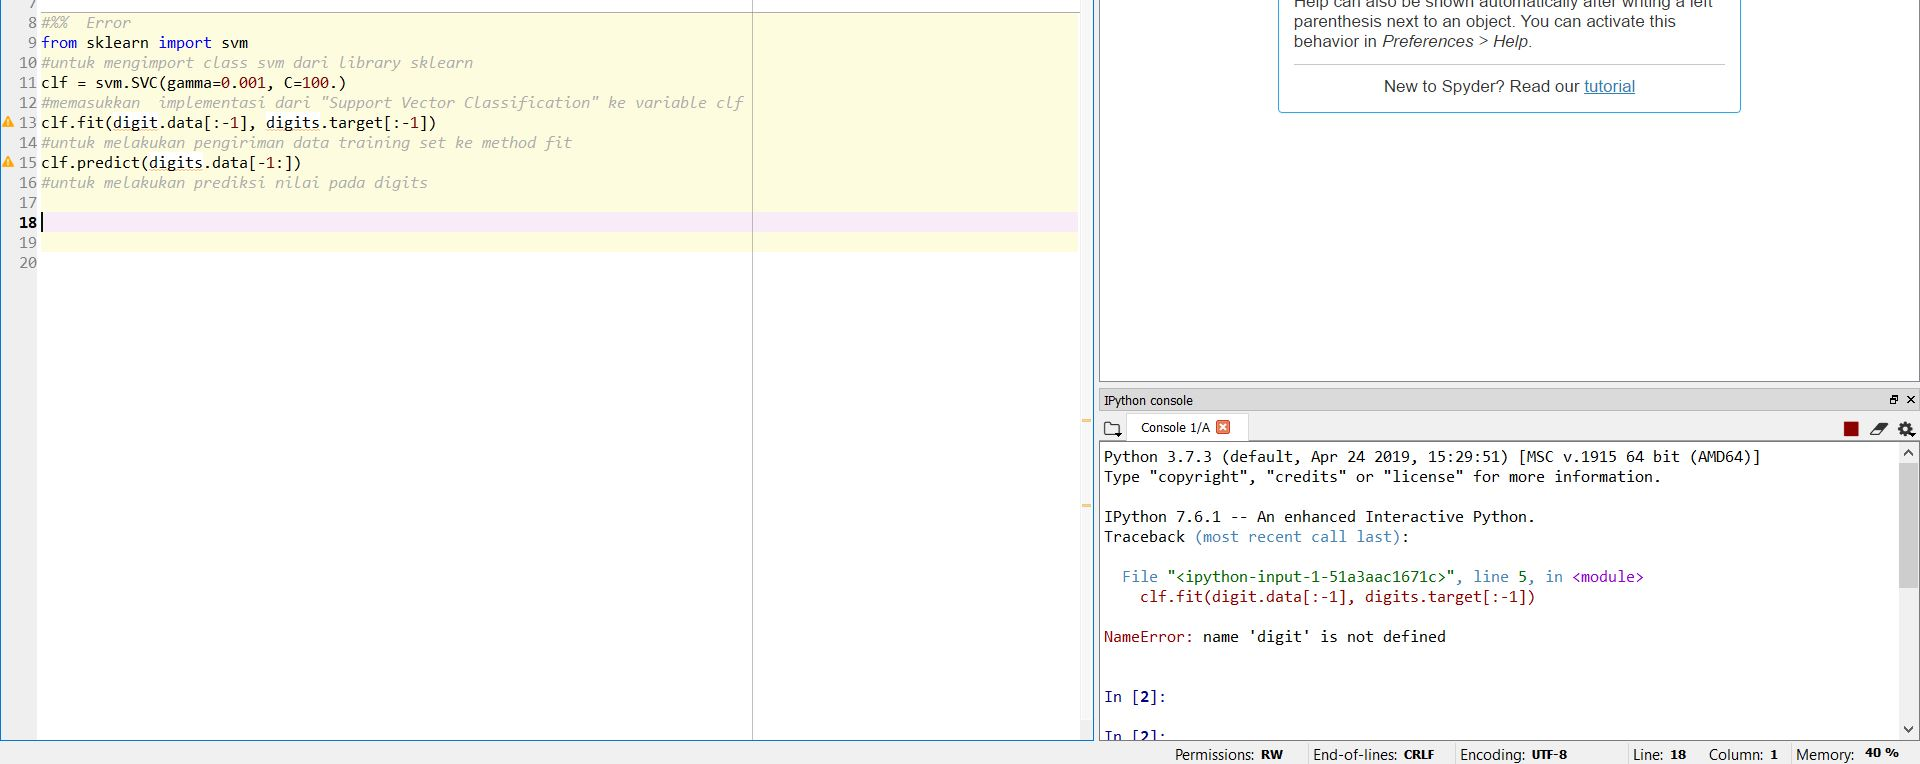
\includegraphics[width=15cm]{figures/1184071/chapter1/3.JPG}
		\centering
		\caption{Name Error}
	\end{figure}
	\newpage\item Tuliskan Kode Error dan Jenis Error
	\hfill\break
	\lstinputlisting[firstline=83, lastline=91]{src/tugas1.py}
\hfill\break
	\item Cara Penangan Error
\hfill\break Tambahkan variabel digits agar kode program dapat terbaca
	\end{enumerate}
	\subsection{Bukti Tidak Plagiarisme}
\begin{figure}[h]
	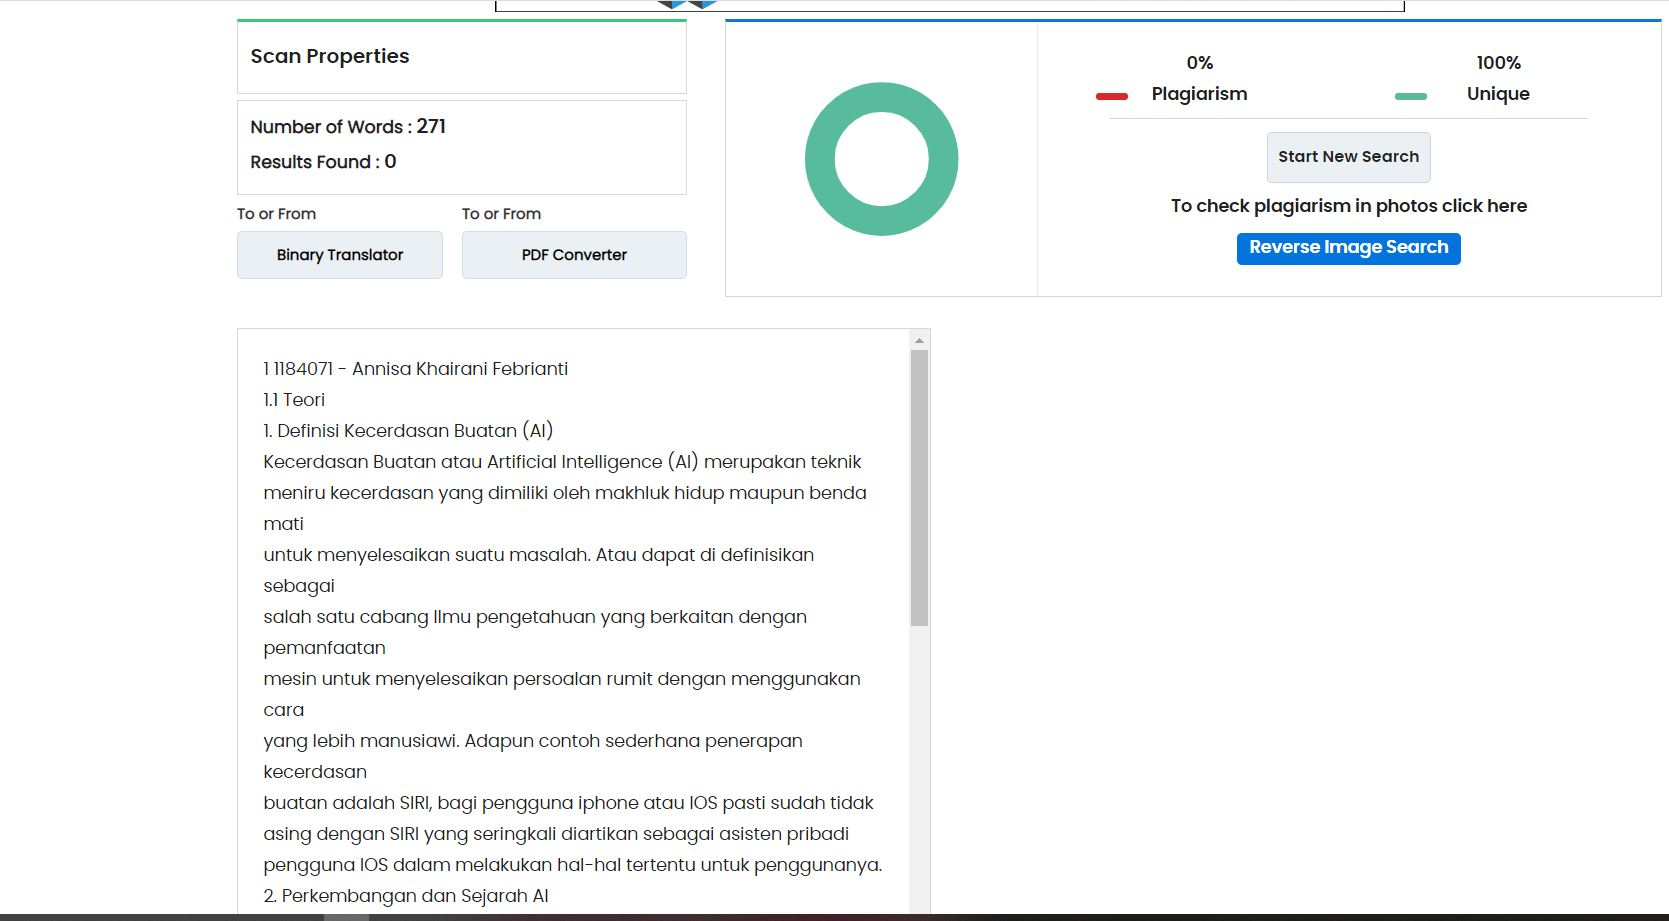
\includegraphics[width=15cm]{figures/1184071/chapter1/4.JPG}
	\centering
	\caption{Bukti Tidak Melakukan Plagiarisme Chapter 1}
\end{figure}
%\chapter{Heriyanto - 1184023}

\section{Teori}

\subsection{Definisi dan Sejarah Kecerdasan Buatan}

\subsubsection{Definisi Kecerdasan Buatan}
Kecerdasan buatan adalah sistem kecerdasan yang ditanamkan atau ditambahkan ke dalam teknologi oleh manusia, yang kemudian akan dikembangkan dalam lingkungan ilmiah atau dalam pembentukan entitas ilmiah yang ada. Kecerdasan di sini menekankan pada kemampuan memperoleh pengetahuan baru, yang dapat langsung diterapkan. Meskipun AI memiliki konotasi ilmiah, AI juga merupakan cabang dari ilmu komputer, pembelajaran, perilaku (behaviour), dan adaptasi pada mesin. \cite{purwanti2017analisis}. 

\subsubsection{Definisi Kecerdasan Buatan Menurut Para Ahli}
\begin{enumerate}
    \item Scahlkoff (1990)
    
    \par Kecerdasan Buatan merupakan bidang studi yang berusaha menerangkan dan meniru perilaku kecerdasan dalam bentuk proses komputasi.\cite{ai2011kecerdasan}
    
    \item Luger dan Stubblefield (1993)
    
    \par Kecerdasan Buatan merupakan cabang ilmu komputer yang berhubungan dengan otomatisasi perilaku yang cerdas.\cite{ai2011kecerdasan}
    
    \item Rich dan Knight (1991)
    
    \par Kecerdasan Buatan merupakan studi tentang cara membuat komputer melakukan sesuatu yang sampai saat ini, orang dapat melakukannya lebih baik.\cite{ai2011kecerdasan}
    
    \item Haag dan Keen (1996)
    
    \par Kecerdasan Buatan adalah bidang studi yang berhubungan dengan penangkapan, pemodelan, dan penyimpanan kecerdasan manusia dalam sebuah sistem teknologi sehingga sistem tersebut dapat memfasilitasi proses pengambilan keputusan yang biasanya dilakukan oleh manusia.\cite{ai2011kecerdasan}
\end{enumerate}

\subsection{Sejarah Kecerdasan Buatan}

\par Istilah kecerdasan buatan pertama kali diusulkan pada tahun 1956. Hingga saat ini, dengan peningkatan daya komputasi dan kapasitas penyimpanan, penggunaan kecerdasan buatan menjadi semakin populer. Fase penelitian awal proyek AI berlangsung sekitar tahun 1950-an, bertujuan untuk mengeksplorasi tema pemecahan masalah dan metode simbolik.

\par Pada 1960-an, Departemen Pertahanan AS juga sangat ingin mengembangkan dan melatih komputer dengan kemampuan dasar penalaran manusia. Sekitar tahun 1970-an, proyek DARPA (Defense Advanced Research Projects Agency) berhasil menyelesaikan studi kasus pemetaan jalan. Di awal abad ke-21, tepatnya tahun 2003, DARPA juga berhasil melahirkan asisten pribadi yang cerdas.

\par Setelah itu, teknologi kecerdasan buatan terus berkembang, dan hingga saat ini memasuki prosedur yang lebih detail dengan menerapkan algoritma deep learning. Di sana, kecerdasan buatan yang dikembangkan dapat melakukan tugas dan memberikan solusi yang lebih kompleks dengan kondisi yang lebih beragam.\cite{sejarahai}

\subsection{Supervised Learning dan Unsupervised Learning}

\subsubsection{Supervised Learning}

\par Supervised learning (pembelajaran terarah) adalah metode pembelajaran mesin di mana pengguna mengharapkan hasil, dan informasinya diketahui atau dimiliki oleh sistem. Artinya metode pembelajaran bekerja dengan menggunakan kembali masukan atau data pengguna dan hasil keluaran yang sebelumnya diselesaikan oleh sistem. Supervised Learning itu sendiri dapat dibagi lagi menjadi regresi dan klasifikasi.\cite{mahardhika2018analisis}

\par Regresi adalah teknik analisis yang digunakan untuk mengidentifikasi hubungan antara dua variabel atau lebih. Tujuan dari regresi adalah untuk menemukan fungsi yang memodelkan data dengan meminimalkan kesalahan atau perbedaan antara nilai prediksi dan nilai sebenarnya.

\par Klasifikasi adalah teknik yang digunakan untuk mengklasifikasikan beberapa item yang tidak berlabel ke dalam satu set kelas diskrit. Klasifikasi mencoba mempelajari hubungan antara sekumpulan variabel fitur dan variabel target. Dalam klasifikasi, variabel targetnya adalah tipe kategori.

\subsubsection{Unsupervised Learning}

\par Unsupervised Learning adalah metode lain dalam materi pembelajaran mesin, di mana tidak ada yang bisa mengetahui hasil yang diharapkan. Tujuan utama dari metode pembelajaran ini adalah agar para penggunanya dapat mengelompokkan objek-objek yang dianggap serupa pada suatu ruang atau area tertentu.\cite{unsuper}

\subsection{Data Set}

\par Kumpulan data adalah objek yang mirip dengan kamus, yang menyimpan semua data dan beberapa metadata tentang data.\cite{scikit} 

\par Saat membuat model Machine Learning, data harus dibagi menjadi satu Training Set dan satu Testing Set. Machine Learning harus diberi tahu "Data Set" mana yang akan dicapai, dan "Data Set" yang dapat digunakan untuk mencapai tujuan. "Data Set" untuk dicapai ini adalah Testing Set, dan "Data Set" untuk mencapai ini disebut Training Set.\cite{dataset}

\par Training Set adalah bagian dari Data Set yang dilatih untuk membuat prediksi atau menjalankan fungsi algoritma ML. Dengan memberikan petunjuk melalui algoritma sehingga mesin yang dilatih dapat menemukan korelasinya sendiri atau mempelajari pola dari data yang diberikan. Testing Set adalah bagian dari data set yang diuji untuk melihat akurasinya, atau dengan kata lain, untuk melihat performanya.\cite{traintest}

\section{Instalasi}

\subsection{Instalasi Scikit-Learn pada Anaconda}

\begin{enumerate}
    \item Pastikan Anaconda telah terpasang pada perangkat komputer atau laptop yang anda gunakan.
    \item Jika Anaconda belum terpasang pada perangkat anda silahkan kunjungi link berikut untuk tutorial memasang anaconda: https://docs.anaconda.com/anaconda/install/.
    \item Setelah anaconda terpasang buka command shell anaconda, dengan mengetik di start menu "Anaconda Prompt (ananconda 3)".
        \begin{figure}[H]
        \centering
        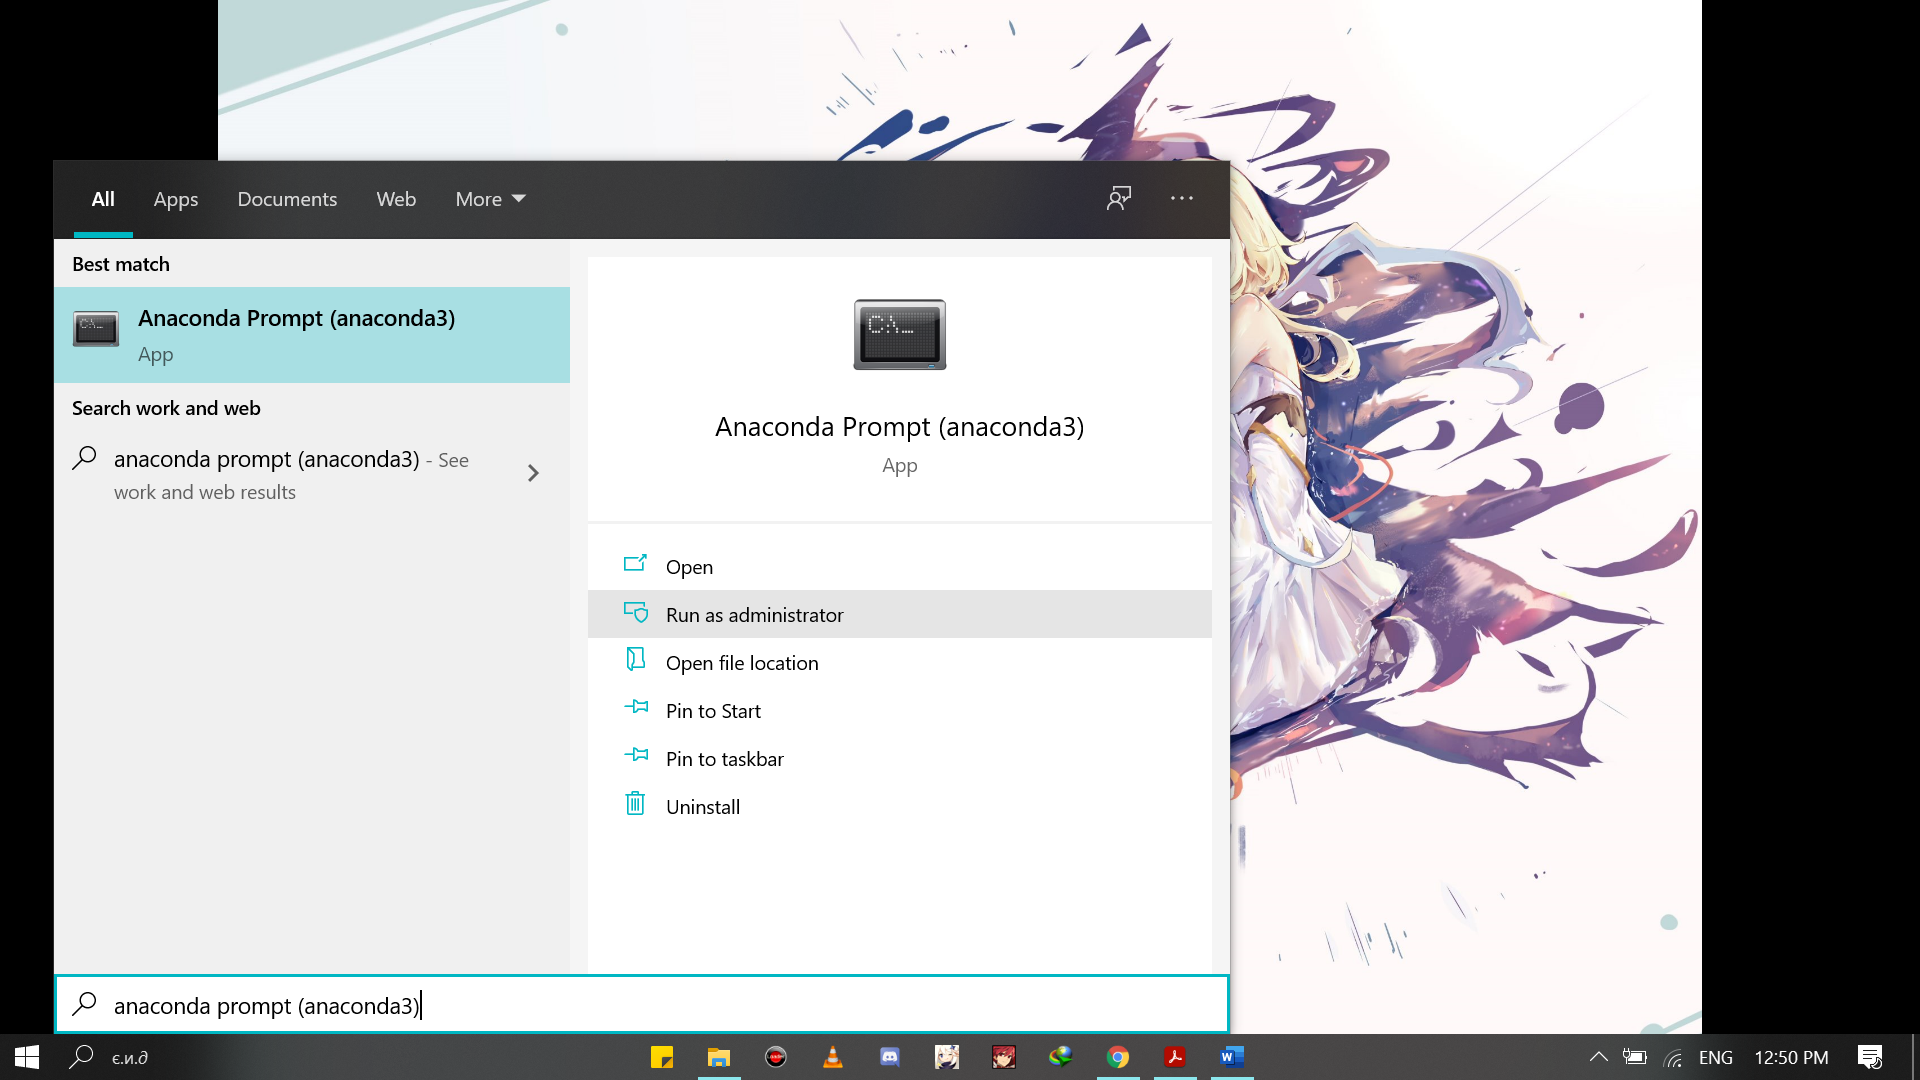
\includegraphics[width=11cm]{figures/1184023/install.png}
        \caption{Anaconda Prompt}
        \end{figure}
    \item Kemudian ketik perintah berikut untuk memasang scikit-learn library pada anaconda: conda install -c conda-forge scikit-learn, dan tunggu sampai prosesnya selesai.
        \begin{figure}[H]
        \centering
        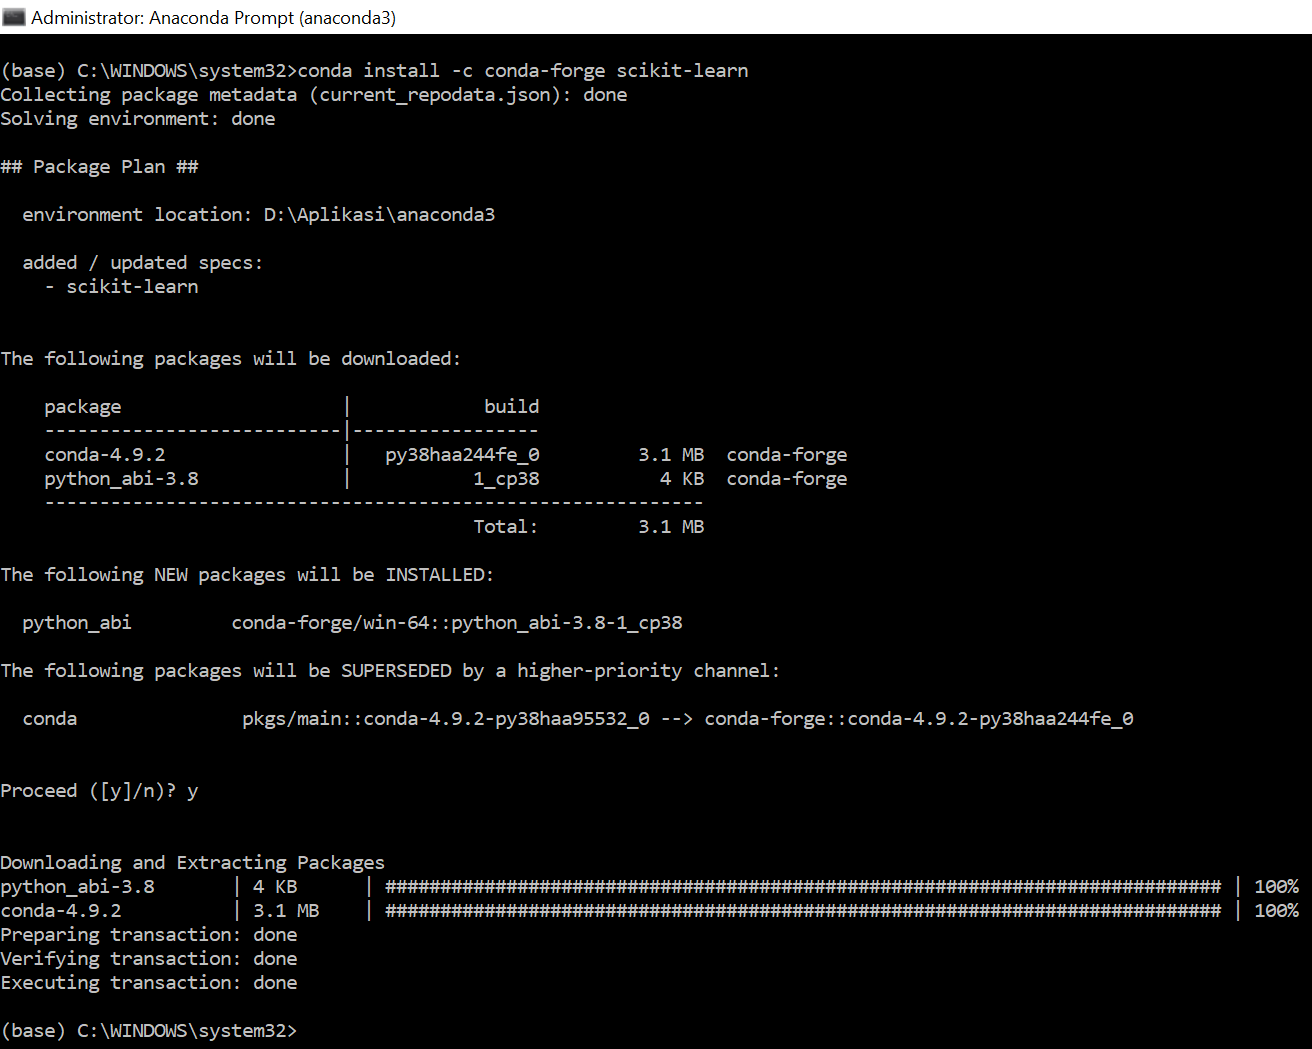
\includegraphics[width=13cm]{figures/1184023/1.PNG}
        \caption{Anaconda Prompt}
        \end{figure}
\end{enumerate}

\subsection{Loading an example dataset}

\par Scikit-learn hadir dengan beberapa dataset standar, misalnya dataset iris dan digit untuk klasifikasi dan dataset diabetes untuk regresi. Berikut ini, dimulai dengan interpreter Python menggunakan tool Spyder kemudian memuat set data iris dan digit.\cite{scikit}
    \begin{figure}[H]
    \centering
    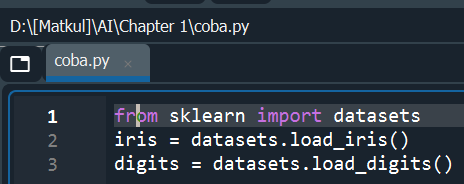
\includegraphics[width=12cm]{figures/1184023/2.PNG}
    \caption{Loading an example dataset}
    \end{figure}

\par Keterangan
    \begin{enumerate}
        \item Baris pertama: meng-import module datasets dari library sklearn.
        \item Baris kedua: iris adalah sebuah variabel dengan nilai yang memuat dataset iris dataset iris.
        \item Baris ketiga: digits adalah sebuah variabel dengan nilai yang memuat dataset digits.
    \end{enumerate}

\par Jika kode tersebut dijalankan akan menghasilkan dataset iris dan digits yang telah dimuat didalam module datasets. Berikut hasil kode yang berjalan tanpa error. Dapat dilihat pada kolom value bahwa dataset-nya telah dimuat.
    \begin{figure}[H]
    \centering
    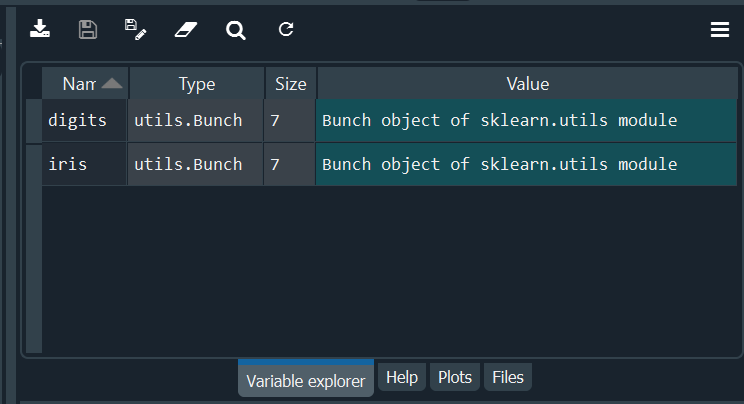
\includegraphics[width=12cm]{figures/1184023/3.PNG}
    \caption{Hasil Dataset}
    \end{figure}

\par Misalnya, untuk kumpulan data digit, Anda dapat menggunakan digits.data untuk mengakses fungsi yang dapat digunakan untuk mengklasifikasikan sampel digit:
    \begin{figure}[H]
    \centering
    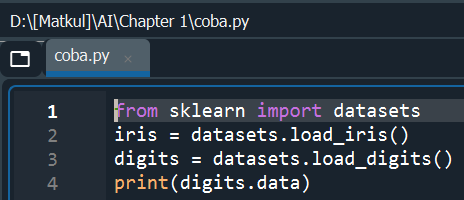
\includegraphics[width=12cm]{figures/1184023/4.PNG}
    \caption{Digits Data}
    \end{figure}

\par Disini kita menambahkan satu baris, yaitu print(digits.data) yang akan menampilkan sampel data digit. Berikut Hasilnya:
    \begin{figure}[H]
    \centering
    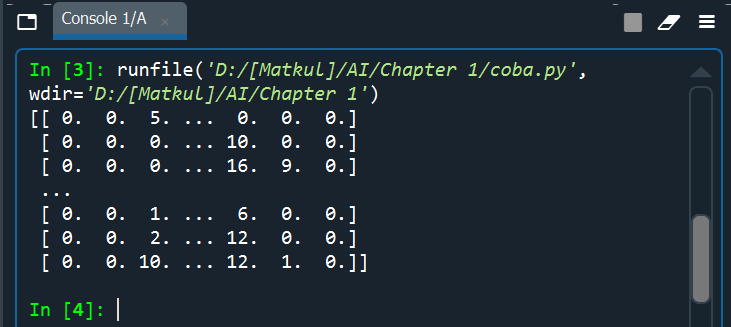
\includegraphics[width=13cm]{figures/1184023/5.PNG}
    \caption{Hasil Digits Data}
    \end{figure}
    
\par Selain digits.data, digits.target memberikan informasi dasar dari kumpulan data digit, yaitu nomor yang sesuai dengan setiap gambar digit yang ingin kita pelajari, berikut kodenya:
    \begin{figure}[H]
    \centering
    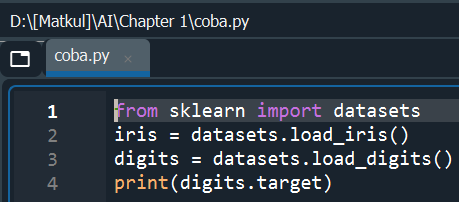
\includegraphics[width=13cm]{figures/1184023/6.PNG}
    \caption{Digits Target}
    \end{figure}

\par Seperti yang dijelaskan diatas sebelumnya digits.target akan memberikan informasi nomor setiap gambar digit yang akan dipelajari. Berikut hasilnya:
    \begin{figure}[H]
    \centering
    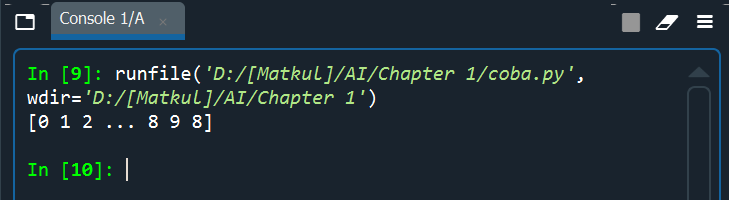
\includegraphics[width=13cm]{figures/1184023/7.PNG}
    \caption{Hasil Digits Target}
    \end{figure}

\par Meskipun data asli mungkin memiliki bentuk yang berbeda, datanya selalu berupa 2D (n-samples, n-features). Untuk digit, setiap sampel asli adalah gambar bentuk (8, 8), yang dapat diakses dengan cara berikut:
    \begin{figure}[H]
    \centering
    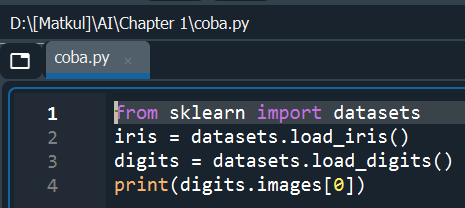
\includegraphics[width=13cm]{figures/1184023/8.PNG}
    \caption{Hasil Digits Target}
    \end{figure}

\par digits.image[0] akan menampilkan digit gambar index ke nol, yang akan menampilkan angka-angka dalam bentuk array.
    \begin{figure}[H]
    \centering
    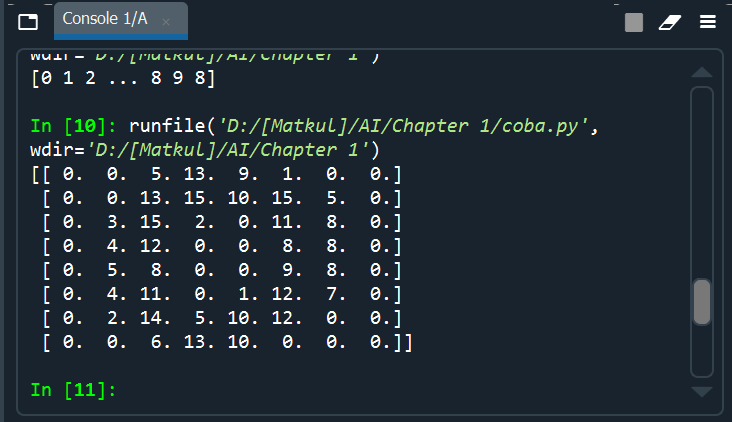
\includegraphics[width=13cm]{figures/1184023/9.PNG}
    \caption{Hasil Digits Image}
    \end{figure}

\subsection{Learning and Predicting}

\par Dalam scikit-learn, estimator yang digunakan untuk klasifikasi adalah objek Python yang mengimplementasikan metode fit (X, y) dan prediksi (T). Contoh prediktor adalah kelas sklearn.svm.SVC, yang mengimplementasikan support vector classification. Estimasi konstruktor diambil sebagai fungsi dari model parameter.

    \begin{figure}[H]
    \centering
    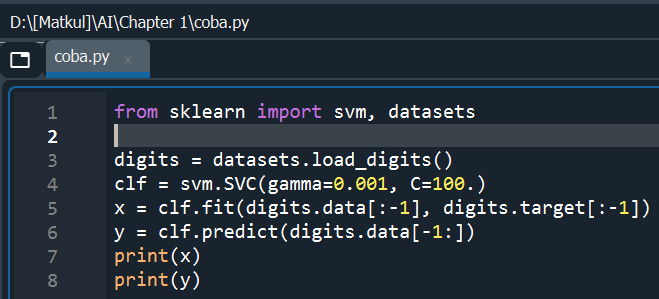
\includegraphics[width=13cm]{figures/1184023/12.PNG}
    \caption{Learning and Predicting}
    \end{figure}

\par Keterangan

    \begin{enumerate}
        \item Baris pertama mengambil module svm dan datasets dari library sklearn.
        \item Baris ketiga adalah variable dengan nama digits yang memiliki nilai untuk memuat dataset digit.
        \item Baris keempat variable clf yang memiliki value gamma=0.001 dan Classification = 100.
        \item Baris kelima variable x yang berisi clf sebagai classifier kemudian fit sebagai method yang mengambil data yang pas dari digits.data dan digits.target dengan nilai training set [:-1].
        \item Baris keenam varible y yang berisi clf sebagai classifier kemudian method predict akan memprediksi digits.data dengan nilai training set [-1:].
        \item Baris ketujuh dan kedelapan akan menampilkan hasil dari method fit dan predict.
    \end{enumerate}

\par Hasil dari method fit dan predict

    \begin{figure}[H]
    \centering
    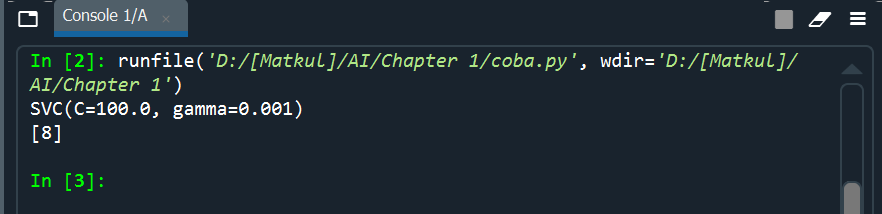
\includegraphics[width=13cm]{figures/1184023/13.PNG}
    \caption{Hasil Learning and Predicting}
    \end{figure}

\subsection{Conventions}

\subsubsection{Type Casting}

    \begin{figure}[H]
    \centering
    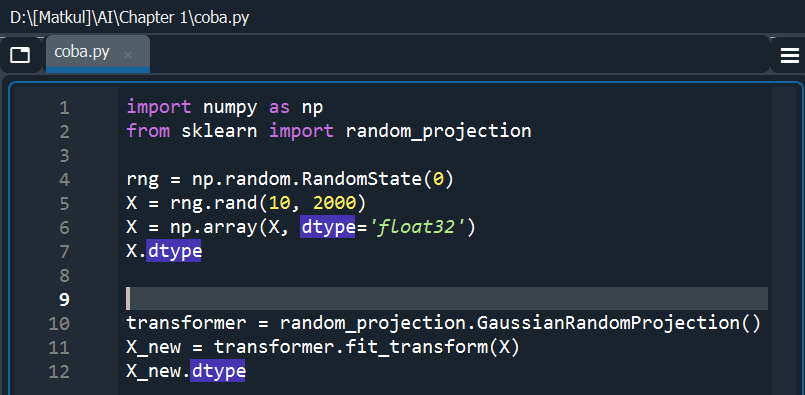
\includegraphics[width=13cm]{figures/1184023/15.PNG}
    \caption{Hasil Learning and Predicting}
    \end{figure}
    
\par Keterangan
    \begin{enumerate}
        \item Baris pertama memanggil library numpy dan dibuat dengan alias np.
        \item Baris kedua memanggil module random projection dari library sklearn.
        \item Baris keempat adalah variable rng yang mendefinisikan numpy as np, kemudian fungsi random dan attr RandomState.
        \item Baris kelima adalah variable X yang mendefinisikan variable rng, kemudian method random yang akan menentukan nilai random dari 10 - 2000.
        \item Baris keenam adalah variable X yang akan menampung nilai random sebelumnya kedalam array dengan tipe data float32.
        \item Baris ketujuh, akan mengubah tipe data nilai random float32 ke float64.
        \item Baris kesepuluh adalah sebuah variable transformer yang mendefinisikan class random projection dan memanggil fungsi GaussianRandomProjection.
        \item Baris kesebelas adalah variable X new yang akan melakukan perhitungan pada variable X.
        \item Baris keduabelas, merubah tipe data menjadi float64.
    \end{enumerate}

\par Hasil dari method X dan X new.

    \begin{figure}[H]
    \centering
    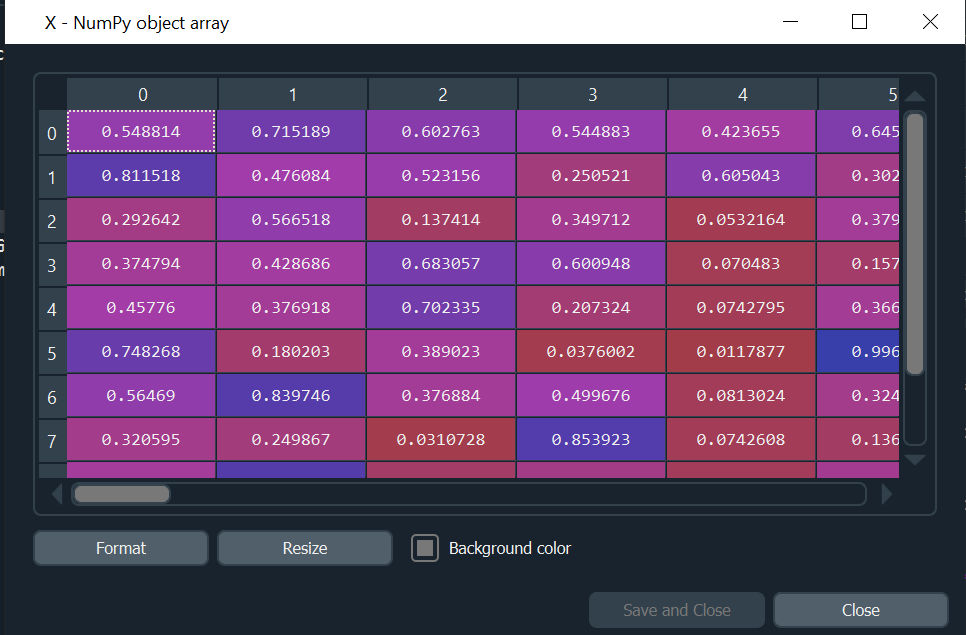
\includegraphics[width=13cm]{figures/1184023/17.PNG}
    \caption{Hasil X Numpy}
    \end{figure}
    
    \begin{figure}[H]
    \centering
    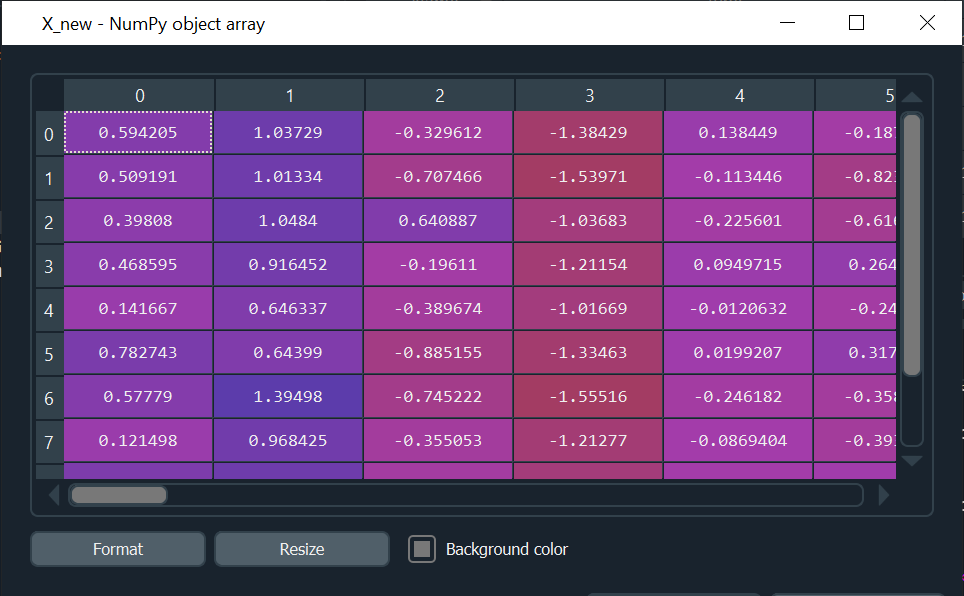
\includegraphics[width=13cm]{figures/1184023/18.PNG}
    \caption{Hasil X new Numpy}
    \end{figure}
    
\par Di sini, predict () pertama kali mengembalikan array integer, karena iris.target (array integer) digunakan dengan tepat. Prediction () kedua mengembalikan larik string karena iris.target names cocok untuk penginstalan.

    \begin{figure}[H]
    \centering
    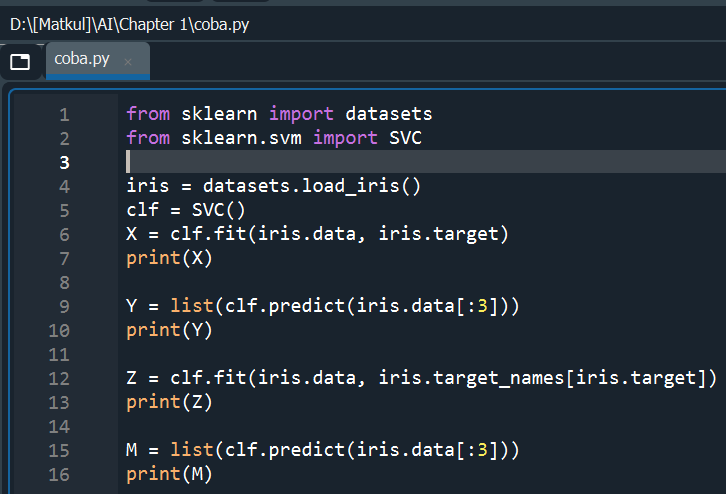
\includegraphics[width=13cm]{figures/1184023/22.PNG}
    \caption{Iris Predict}
    \end{figure}

\par Keterangan 
    \begin{enumerate}
        \item Baris pertama, memanggil module datasets dari library sklearn.
        \item Baris kedua, memanggil module SVC dari library sklearn.svm.
        \item Baris keempat, variable iris yang memuat datasets iris.
        \item Baris kelima, variable clf yang memanggil method SVC.
        \item Baris keenam, variable X yang memanggil classifier kemudian method fit yang memanggil data pas dari iris.data dan target.
        \item Baris ketujuh, menampilkan hasil variable X.
        \item Baris kesembilan, variable Y yang akan mengembalikan iris predict dalam bentuk array.
        \item Baris kesepuluh, menampilkan hasil variable Y.
        \item Baris keduabelas, memanggil classifier kemudian method fit yang memanggil data pas dari iris.names, iris.data, dan target.
        \item Baris ketigabelas, menampilkan hasil variable Z.
        \item Baris kelimabelas, variable M yang akan mengembalikan iris predict kedalam bentuk string.
        \item keenambelas, menampilkan hasil variable M.
    \end{enumerate}

\par Hasil dari iris predict.

    \begin{figure}[H]
    \centering
    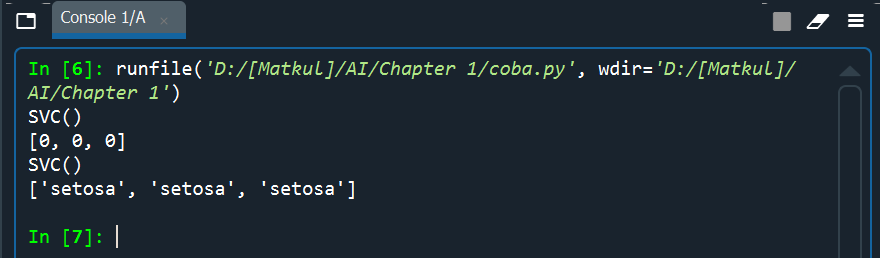
\includegraphics[width=13cm]{figures/1184023/23.PNG}
    \caption{Hasil Iris Predict}
    \end{figure}
    
\par Di sini, predict () pertama kali mengembalikan array integer, karena iris.target (array integer) digunakan dengan tepat. Prediction () kedua mengembalikan string karena iris.targetnames cocok untuk penginstalan.

\subsubsection{Refitting and updating parameters}

\par Hyperparameter dari estimator dapat diperbarui setelah dibuat dengan metode setparams (). Memanggil fit () beberapa kali akan menimpa fit () yang dipelajari sebelumnya:

    \begin{figure}[H]
    \centering
    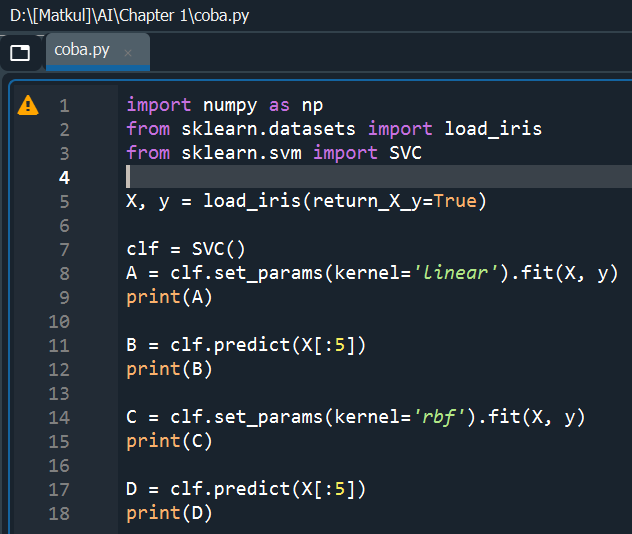
\includegraphics[width=13cm]{figures/1184023/24.PNG}
    \caption{Refitting and updating parameters}
    \end{figure}

\par Keterangan:
    \begin{enumerate}
        \item Baris pertama, memanggil library numpy dengan alias np.
        \item Baris kedua, memanggil module load iris dari library sklearn.datasets.
        \item Baris ketiga, memanggil module SVC dari library sklearn.svm.
        \item Baris kelima, mengisi variable X dan y dengan datasets iris.
        \item Baris ketujuh, mendifinisikan clf sebagai fungsi SVC.
        \item Baris kedelapan, mengubah rbf menjadi linear melalui SVC.setparams kedalam variable A.
        \item Baris kesembilan, menampilkan hasil variable A.
        \item Baris kesebelas, clf dengan method predict akan menampilkan data X dalam array sebanyak 5 data kedalam variable B.
        \item Baris keduabelas, menampilkan hasil variable B.
        \item Baris keempatbelas, mengubah linear ke rbf melalui SVC.setparams kedalam variable C.
        \item Baris kelimabelas, menampilkan hasil variable C.
        \item Baris ketujuhbelas, clf dengan method predict akan menampilkan data X dalam array sebanyak 5 data kedalam variable D.
        \item Baris kedelapanbelas, menampilkan hasil variable D.
    \end{enumerate}

\par Hasil dari Refitting and updating parameters.

    \begin{figure}[H]
    \centering
    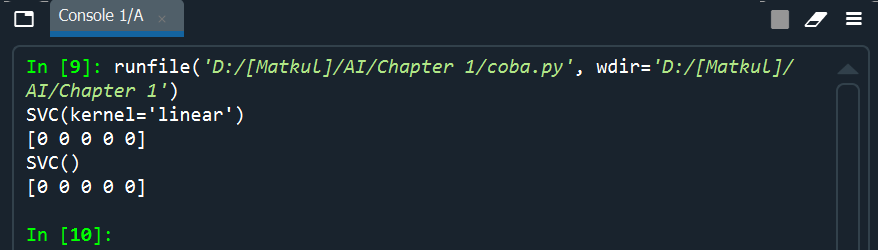
\includegraphics[width=13cm]{figures/1184023/25.PNG}
    \caption{Hasil Refitting and updating parameters}
    \end{figure}

\par Di sini, kernel default rbf pertama-tama diubah menjadi linier oleh SVC.setparams () setelah membuat estimator, dan kemudian diubah kembali ke rbf untuk mereparasi estimator dan membuat prediksi kedua.

\subsubsection{Multiclass vs. multilabel fitting}

\par Saat menggunakan multiclass classifiers, tugas learning and prediction yang dilakukan bergantung pada format data target yang sesuai, yang bergantung pada:

    \begin{figure}[H]
    \centering
    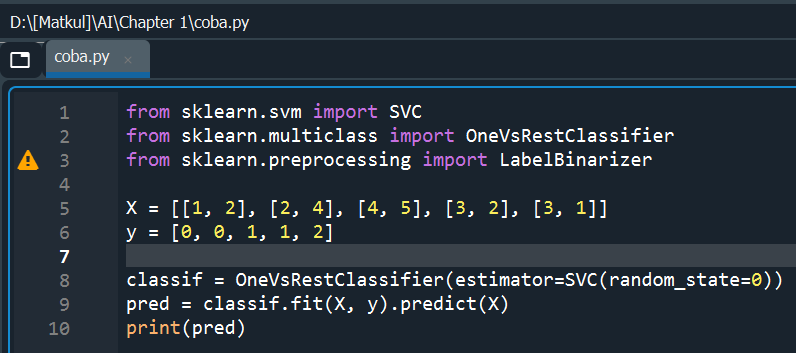
\includegraphics[width=13cm]{figures/1184023/26.PNG}
    \caption{Multiclass Predict}
    \end{figure}

\par Keterangan:
    \begin{enumerate}
        \item Baris pertama, memanggil module SVC dari library sklearn.svm.
        \item Baris kedua, memanggil module OneVsRestClassifier dari library sklearn.multiclass.
        \item Baris ketiga, memanggil module LabelBinarizer dari library sklearn.preprocessing.
        \item Baris kelima dan keenam, variable x dan y yang berisi data array.
        \item Baris kedelapan, menggunakan method OneVsRestClassifier dengan fungsi SVC sebagai estimator untuk menghasilkan data random yang didefiniskan kedalam classif.
        \item Baris kesembilan, memberikan hasil multiclass prediksi yang sesuai kedalam variable pred.
        \item Baris kesepuluh, menampilkan hasil variable pred.
    \end{enumerate}

\par Hasil dari Multiclass Predict.

    \begin{figure}[H]
    \centering
    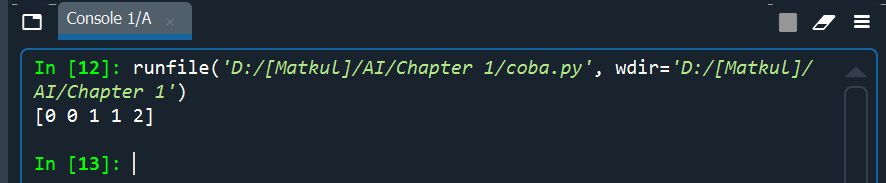
\includegraphics[width=13cm]{figures/1184023/27.PNG}
    \caption{Hasil Multiclass Predict}
    \end{figure}

\par Dalam kasus di atas, classifier cocok untuk pred label multiclass, sehingga metode predict () menyediakan prediksi multiclass yang sesuai. Dimungkinkan juga untuk menyesuaikan dengan array 2d indikator label biner:

    \begin{figure}[H]
    \centering
    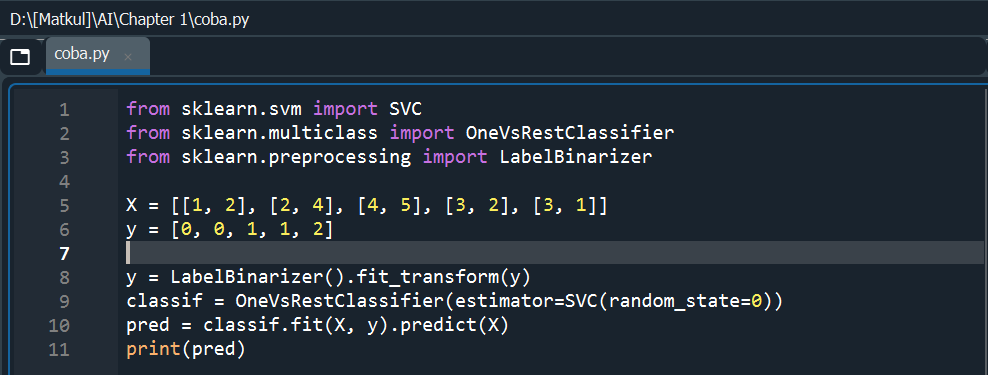
\includegraphics[width=13cm]{figures/1184023/28.PNG}
    \caption{Multiclass Predict 2}
    \end{figure}
    
\par Keterangan:
    \begin{enumerate}
        \item Baris pertama, memanggil module SVC dari library sklearn.svm.
        \item Baris kedua, memanggil module OneVsRestClassifier dari library sklearn.multiclass.
        \item Baris ketiga, memanggil module LabelBinarizer dari library sklearn.preprocessing.
        \item Baris kelima dan keenam, variable x dan y yang berisi data array.
        \item Baris kedelapan, classifier fit() merepresentasi variable y dengan LabelBinarizer.
        \item Baris kesembilan, menggunakan method OneVsRestClassifier dengan fungsi SVC sebagai estimator untuk menghasilkan data random yang didefiniskan kedalam classif.
        \item Baris kesepuluh, memberikan hasil multiclass prediksi yang sesuai kedalam variable pred.
        \item Baris kesebelas, menampilkan hasil variable pred. 
    \end{enumerate}

\par Hasil dari Multiclass Predict 2

    \begin{figure}[H]
    \centering
    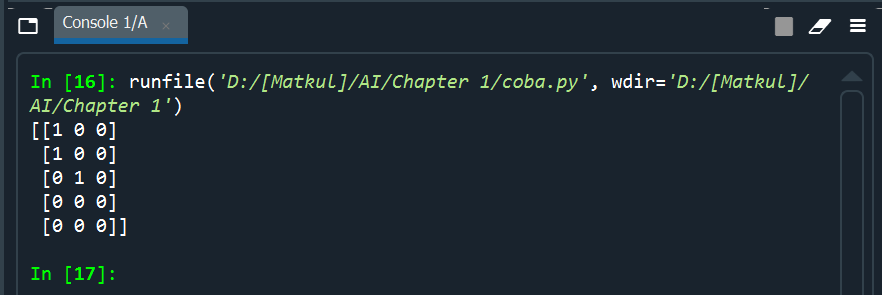
\includegraphics[width=13cm]{figures/1184023/29.PNG}
    \caption{Hasil Multiclass Predict 2}
    \end{figure}

\par Di sini, LabelBinarizer digunakan untuk menyesuaikan pengklasifikasi dengan representasi label biner pred dari y. Dalam kasus ini, predict () mengembalikan pred dalam bentuk array yang mewakili prediksi yang sesuai.

\par MultiLabel Fitting, dalam kasus ini, beberapa label ditetapkan ke classifier yang sesuai untuk setiap sampel. MultiLabelBinarizer digunakan untuk membuat binarisasi pred multilabel agar sesuai. Akibatnya, predict () mengembalikan larik pred yang berisi beberapa label yang diprediksi untuk setiap instance.

    \begin{figure}[H]
    \centering
    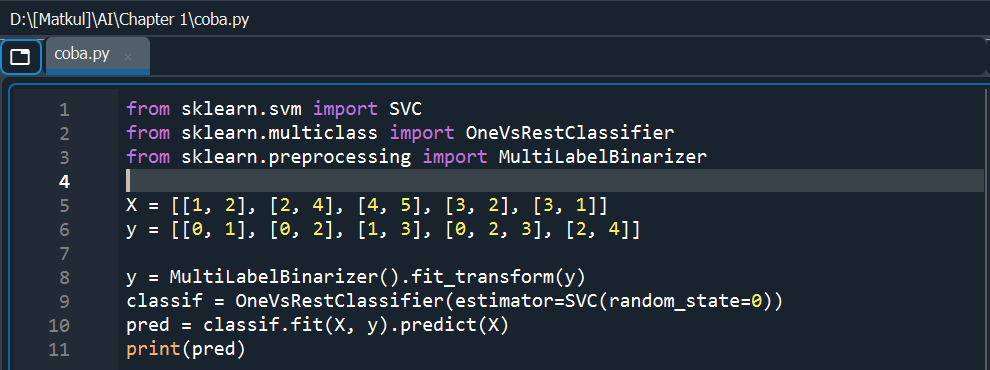
\includegraphics[width=13cm]{figures/1184023/30.PNG}
    \caption{MultiLabel Fitting}
    \end{figure}

\par Keterangan:
    \begin{enumerate}
        \item Baris pertama, memanggil module SVC dari library sklearn.svm.
        \item Baris kedua, memanggil module OneVsRestClassifier dari library sklearn.multiclass.
        \item Baris ketiga, memanggil module LabelBinarizer dari library sklearn.preprocessing.
        \item Baris kelima dan keenam, variable x dan y yang berisi data array.
        \item Baris kedelapan, classifier fit() merepresentasi variable y dengan MultiLabelBinarizer.
        \item Baris kesembilan, menggunakan method OneVsRestClassifier dengan fungsi SVC sebagai estimator untuk menghasilkan data random yang didefiniskan kedalam classif.
        \item Baris kesepuluh, memberikan hasil multiclass prediksi yang sesuai kedalam variable pred.
        \item Baris kesebelas, menampilkan hasil variable pred. 
    \end{enumerate}

\par Hasil dari Multilabel Fitting

    \begin{figure}[H]
    \centering
    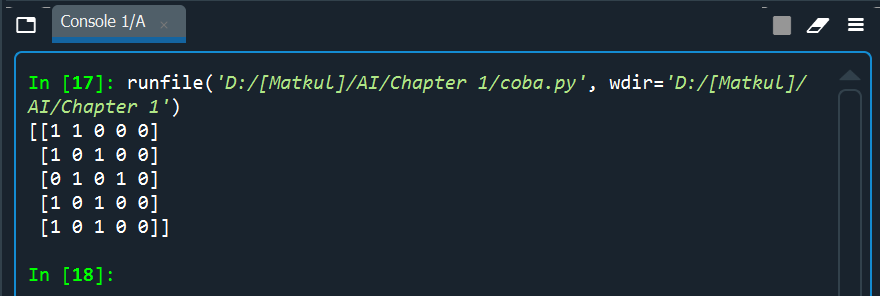
\includegraphics[width=13cm]{figures/1184023/31.PNG}
    \caption{Hasil MultiLabel Fitting}
    \end{figure}

\section{Penanganan Error}

\subsection{Error 1}

    \begin{figure}[H]
    \centering
    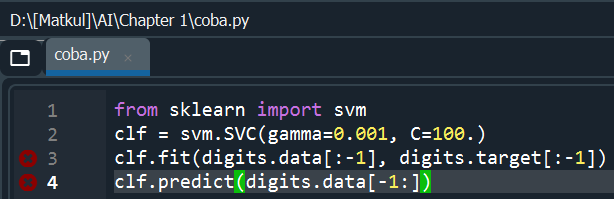
\includegraphics[width=13cm]{figures/1184023/error/1.PNG}
    \caption{Hasil MultiLabel Fitting}
    \end{figure}

\par Pada baris tiga dan empat terdapat error, yaitu sebagai berikut:

    \begin{figure}[H]
    \centering
    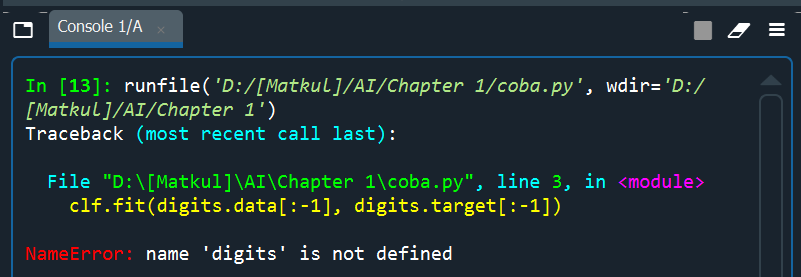
\includegraphics[width=13cm]{figures/1184023/error/2.PNG}
    \caption{Hasil MultiLabel Fitting}
    \end{figure}

\par Nama errornya adalah karena "digits" tidak terdifinisikan. Untuk penanganannya kita harus mendefinisikan digits sebagai berikut:

    \begin{figure}[H]
    \centering
    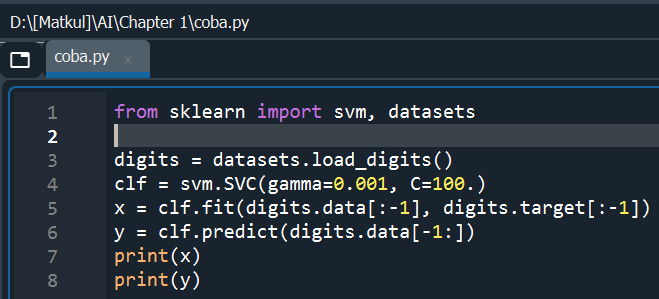
\includegraphics[width=13cm]{figures/1184023/12.PNG}
    \caption{Learning and Predicting}
    \end{figure}

\par Dapat dilihat perbedaannya pada baris pertama dan ketiga, pada baris pertama, memanggil modul datasets yang sebelumnya tidak ada dan kemudian pada baris ketiga, digits didefinisikan.



\bibliographystyle{IEEEtran} 
%\def\bibfont{\normalsize}
\bibliography{references}


%%%%%%%%%%%%%%%
%%  The default LaTeX Index
%%  Don't need to add any commands before \begin{document}
\printindex

%%%% Making an index
%% 
%% 1. Make index entries, don't leave any spaces so that they
%% will be sorted correctly.
%% 
%% \index{term}
%% \index{term!subterm}
%% \index{term!subterm!subsubterm}
%% 
%% 2. Run LaTeX several times to produce <filename>.idx
%% 
%% 3. On command line, type  makeindx <filename> which
%% will produce <filename>.ind 
%% 
%% 4. Type \printindex to make the index appear in your book.
%% 
%% 5. If you would like to edit <filename>.ind 
%% you may do so. See docs.pdf for more information.
%% 
%%%%%%%%%%%%%%%%%%%%%%%%%%%%%%

%%%%%%%%%%%%%% Making Multiple Indices %%%%%%%%%%%%%%%%
%% 1. 
%% \usepackage{multind}
%% \makeindex{book}
%% \makeindex{authors}
%% \begin{document}
%% 
%% 2.
%% % add index terms to your book, ie,
%% \index{book}{A term to go to the topic index}
%% \index{authors}{Put this author in the author index}
%% 
%% \index{book}{Cows}
%% \index{book}{Cows!Jersey}
%% \index{book}{Cows!Jersey!Brown}
%% 
%% \index{author}{Douglas Adams}
%% \index{author}{Boethius}
%% \index{author}{Mark Twain}
%% 
%% 3. On command line type 
%% makeindex topic 
%% makeindex authors
%% 
%% 4.
%% this is a Wiley command to make the indices print:
%% \multiprintindex{book}{Topic index}
%% \multiprintindex{authors}{Author index}

\end{document}

